% Options for packages loaded elsewhere
\PassOptionsToPackage{unicode}{hyperref}
\PassOptionsToPackage{hyphens}{url}
\PassOptionsToPackage{dvipsnames,svgnames,x11names}{xcolor}
%
\documentclass[
  letterpaper,
  DIV=11,
  numbers=noendperiod]{scrreprt}

\usepackage{amsmath,amssymb}
\usepackage{iftex}
\ifPDFTeX
  \usepackage[T1]{fontenc}
  \usepackage[utf8]{inputenc}
  \usepackage{textcomp} % provide euro and other symbols
\else % if luatex or xetex
  \usepackage{unicode-math}
  \defaultfontfeatures{Scale=MatchLowercase}
  \defaultfontfeatures[\rmfamily]{Ligatures=TeX,Scale=1}
\fi
\usepackage{lmodern}
\ifPDFTeX\else  
    % xetex/luatex font selection
\fi
% Use upquote if available, for straight quotes in verbatim environments
\IfFileExists{upquote.sty}{\usepackage{upquote}}{}
\IfFileExists{microtype.sty}{% use microtype if available
  \usepackage[]{microtype}
  \UseMicrotypeSet[protrusion]{basicmath} % disable protrusion for tt fonts
}{}
\makeatletter
\@ifundefined{KOMAClassName}{% if non-KOMA class
  \IfFileExists{parskip.sty}{%
    \usepackage{parskip}
  }{% else
    \setlength{\parindent}{0pt}
    \setlength{\parskip}{6pt plus 2pt minus 1pt}}
}{% if KOMA class
  \KOMAoptions{parskip=half}}
\makeatother
\usepackage{xcolor}
\setlength{\emergencystretch}{3em} % prevent overfull lines
\setcounter{secnumdepth}{5}
% Make \paragraph and \subparagraph free-standing
\makeatletter
\ifx\paragraph\undefined\else
  \let\oldparagraph\paragraph
  \renewcommand{\paragraph}{
    \@ifstar
      \xxxParagraphStar
      \xxxParagraphNoStar
  }
  \newcommand{\xxxParagraphStar}[1]{\oldparagraph*{#1}\mbox{}}
  \newcommand{\xxxParagraphNoStar}[1]{\oldparagraph{#1}\mbox{}}
\fi
\ifx\subparagraph\undefined\else
  \let\oldsubparagraph\subparagraph
  \renewcommand{\subparagraph}{
    \@ifstar
      \xxxSubParagraphStar
      \xxxSubParagraphNoStar
  }
  \newcommand{\xxxSubParagraphStar}[1]{\oldsubparagraph*{#1}\mbox{}}
  \newcommand{\xxxSubParagraphNoStar}[1]{\oldsubparagraph{#1}\mbox{}}
\fi
\makeatother

\usepackage{color}
\usepackage{fancyvrb}
\newcommand{\VerbBar}{|}
\newcommand{\VERB}{\Verb[commandchars=\\\{\}]}
\DefineVerbatimEnvironment{Highlighting}{Verbatim}{commandchars=\\\{\}}
% Add ',fontsize=\small' for more characters per line
\usepackage{framed}
\definecolor{shadecolor}{RGB}{241,243,245}
\newenvironment{Shaded}{\begin{snugshade}}{\end{snugshade}}
\newcommand{\AlertTok}[1]{\textcolor[rgb]{0.68,0.00,0.00}{#1}}
\newcommand{\AnnotationTok}[1]{\textcolor[rgb]{0.37,0.37,0.37}{#1}}
\newcommand{\AttributeTok}[1]{\textcolor[rgb]{0.40,0.45,0.13}{#1}}
\newcommand{\BaseNTok}[1]{\textcolor[rgb]{0.68,0.00,0.00}{#1}}
\newcommand{\BuiltInTok}[1]{\textcolor[rgb]{0.00,0.23,0.31}{#1}}
\newcommand{\CharTok}[1]{\textcolor[rgb]{0.13,0.47,0.30}{#1}}
\newcommand{\CommentTok}[1]{\textcolor[rgb]{0.37,0.37,0.37}{#1}}
\newcommand{\CommentVarTok}[1]{\textcolor[rgb]{0.37,0.37,0.37}{\textit{#1}}}
\newcommand{\ConstantTok}[1]{\textcolor[rgb]{0.56,0.35,0.01}{#1}}
\newcommand{\ControlFlowTok}[1]{\textcolor[rgb]{0.00,0.23,0.31}{\textbf{#1}}}
\newcommand{\DataTypeTok}[1]{\textcolor[rgb]{0.68,0.00,0.00}{#1}}
\newcommand{\DecValTok}[1]{\textcolor[rgb]{0.68,0.00,0.00}{#1}}
\newcommand{\DocumentationTok}[1]{\textcolor[rgb]{0.37,0.37,0.37}{\textit{#1}}}
\newcommand{\ErrorTok}[1]{\textcolor[rgb]{0.68,0.00,0.00}{#1}}
\newcommand{\ExtensionTok}[1]{\textcolor[rgb]{0.00,0.23,0.31}{#1}}
\newcommand{\FloatTok}[1]{\textcolor[rgb]{0.68,0.00,0.00}{#1}}
\newcommand{\FunctionTok}[1]{\textcolor[rgb]{0.28,0.35,0.67}{#1}}
\newcommand{\ImportTok}[1]{\textcolor[rgb]{0.00,0.46,0.62}{#1}}
\newcommand{\InformationTok}[1]{\textcolor[rgb]{0.37,0.37,0.37}{#1}}
\newcommand{\KeywordTok}[1]{\textcolor[rgb]{0.00,0.23,0.31}{\textbf{#1}}}
\newcommand{\NormalTok}[1]{\textcolor[rgb]{0.00,0.23,0.31}{#1}}
\newcommand{\OperatorTok}[1]{\textcolor[rgb]{0.37,0.37,0.37}{#1}}
\newcommand{\OtherTok}[1]{\textcolor[rgb]{0.00,0.23,0.31}{#1}}
\newcommand{\PreprocessorTok}[1]{\textcolor[rgb]{0.68,0.00,0.00}{#1}}
\newcommand{\RegionMarkerTok}[1]{\textcolor[rgb]{0.00,0.23,0.31}{#1}}
\newcommand{\SpecialCharTok}[1]{\textcolor[rgb]{0.37,0.37,0.37}{#1}}
\newcommand{\SpecialStringTok}[1]{\textcolor[rgb]{0.13,0.47,0.30}{#1}}
\newcommand{\StringTok}[1]{\textcolor[rgb]{0.13,0.47,0.30}{#1}}
\newcommand{\VariableTok}[1]{\textcolor[rgb]{0.07,0.07,0.07}{#1}}
\newcommand{\VerbatimStringTok}[1]{\textcolor[rgb]{0.13,0.47,0.30}{#1}}
\newcommand{\WarningTok}[1]{\textcolor[rgb]{0.37,0.37,0.37}{\textit{#1}}}

\providecommand{\tightlist}{%
  \setlength{\itemsep}{0pt}\setlength{\parskip}{0pt}}\usepackage{longtable,booktabs,array}
\usepackage{calc} % for calculating minipage widths
% Correct order of tables after \paragraph or \subparagraph
\usepackage{etoolbox}
\makeatletter
\patchcmd\longtable{\par}{\if@noskipsec\mbox{}\fi\par}{}{}
\makeatother
% Allow footnotes in longtable head/foot
\IfFileExists{footnotehyper.sty}{\usepackage{footnotehyper}}{\usepackage{footnote}}
\makesavenoteenv{longtable}
\usepackage{graphicx}
\makeatletter
\def\maxwidth{\ifdim\Gin@nat@width>\linewidth\linewidth\else\Gin@nat@width\fi}
\def\maxheight{\ifdim\Gin@nat@height>\textheight\textheight\else\Gin@nat@height\fi}
\makeatother
% Scale images if necessary, so that they will not overflow the page
% margins by default, and it is still possible to overwrite the defaults
% using explicit options in \includegraphics[width, height, ...]{}
\setkeys{Gin}{width=\maxwidth,height=\maxheight,keepaspectratio}
% Set default figure placement to htbp
\makeatletter
\def\fps@figure{htbp}
\makeatother
% definitions for citeproc citations
\NewDocumentCommand\citeproctext{}{}
\NewDocumentCommand\citeproc{mm}{%
  \begingroup\def\citeproctext{#2}\cite{#1}\endgroup}
\makeatletter
 % allow citations to break across lines
 \let\@cite@ofmt\@firstofone
 % avoid brackets around text for \cite:
 \def\@biblabel#1{}
 \def\@cite#1#2{{#1\if@tempswa , #2\fi}}
\makeatother
\newlength{\cslhangindent}
\setlength{\cslhangindent}{1.5em}
\newlength{\csllabelwidth}
\setlength{\csllabelwidth}{3em}
\newenvironment{CSLReferences}[2] % #1 hanging-indent, #2 entry-spacing
 {\begin{list}{}{%
  \setlength{\itemindent}{0pt}
  \setlength{\leftmargin}{0pt}
  \setlength{\parsep}{0pt}
  % turn on hanging indent if param 1 is 1
  \ifodd #1
   \setlength{\leftmargin}{\cslhangindent}
   \setlength{\itemindent}{-1\cslhangindent}
  \fi
  % set entry spacing
  \setlength{\itemsep}{#2\baselineskip}}}
 {\end{list}}
\usepackage{calc}
\newcommand{\CSLBlock}[1]{\hfill\break\parbox[t]{\linewidth}{\strut\ignorespaces#1\strut}}
\newcommand{\CSLLeftMargin}[1]{\parbox[t]{\csllabelwidth}{\strut#1\strut}}
\newcommand{\CSLRightInline}[1]{\parbox[t]{\linewidth - \csllabelwidth}{\strut#1\strut}}
\newcommand{\CSLIndent}[1]{\hspace{\cslhangindent}#1}

\KOMAoption{captions}{tableheading}
\makeatletter
\@ifpackageloaded{tcolorbox}{}{\usepackage[skins,breakable]{tcolorbox}}
\@ifpackageloaded{fontawesome5}{}{\usepackage{fontawesome5}}
\definecolor{quarto-callout-color}{HTML}{909090}
\definecolor{quarto-callout-note-color}{HTML}{0758E5}
\definecolor{quarto-callout-important-color}{HTML}{CC1914}
\definecolor{quarto-callout-warning-color}{HTML}{EB9113}
\definecolor{quarto-callout-tip-color}{HTML}{00A047}
\definecolor{quarto-callout-caution-color}{HTML}{FC5300}
\definecolor{quarto-callout-color-frame}{HTML}{acacac}
\definecolor{quarto-callout-note-color-frame}{HTML}{4582ec}
\definecolor{quarto-callout-important-color-frame}{HTML}{d9534f}
\definecolor{quarto-callout-warning-color-frame}{HTML}{f0ad4e}
\definecolor{quarto-callout-tip-color-frame}{HTML}{02b875}
\definecolor{quarto-callout-caution-color-frame}{HTML}{fd7e14}
\makeatother
\makeatletter
\@ifpackageloaded{bookmark}{}{\usepackage{bookmark}}
\makeatother
\makeatletter
\@ifpackageloaded{caption}{}{\usepackage{caption}}
\AtBeginDocument{%
\ifdefined\contentsname
  \renewcommand*\contentsname{Table of contents}
\else
  \newcommand\contentsname{Table of contents}
\fi
\ifdefined\listfigurename
  \renewcommand*\listfigurename{List of Figures}
\else
  \newcommand\listfigurename{List of Figures}
\fi
\ifdefined\listtablename
  \renewcommand*\listtablename{List of Tables}
\else
  \newcommand\listtablename{List of Tables}
\fi
\ifdefined\figurename
  \renewcommand*\figurename{Figure}
\else
  \newcommand\figurename{Figure}
\fi
\ifdefined\tablename
  \renewcommand*\tablename{Table}
\else
  \newcommand\tablename{Table}
\fi
}
\@ifpackageloaded{float}{}{\usepackage{float}}
\floatstyle{ruled}
\@ifundefined{c@chapter}{\newfloat{codelisting}{h}{lop}}{\newfloat{codelisting}{h}{lop}[chapter]}
\floatname{codelisting}{Listing}
\newcommand*\listoflistings{\listof{codelisting}{List of Listings}}
\makeatother
\makeatletter
\makeatother
\makeatletter
\@ifpackageloaded{caption}{}{\usepackage{caption}}
\@ifpackageloaded{subcaption}{}{\usepackage{subcaption}}
\makeatother

\ifLuaTeX
  \usepackage{selnolig}  % disable illegal ligatures
\fi
\usepackage{bookmark}

\IfFileExists{xurl.sty}{\usepackage{xurl}}{} % add URL line breaks if available
\urlstyle{same} % disable monospaced font for URLs
\hypersetup{
  pdftitle={Data Management},
  pdfauthor={Moses Otieno},
  colorlinks=true,
  linkcolor={blue},
  filecolor={Maroon},
  citecolor={Blue},
  urlcolor={Blue},
  pdfcreator={LaTeX via pandoc}}


\title{Data Management}
\author{Moses Otieno}
\date{2024-08-10}

\begin{document}
\maketitle

\renewcommand*\contentsname{Table of contents}
{
\hypersetup{linkcolor=}
\setcounter{tocdepth}{2}
\tableofcontents
}

\bookmarksetup{startatroot}

\chapter*{Preface}\label{preface}
\addcontentsline{toc}{chapter}{Preface}

\markboth{Preface}{Preface}

\section*{What is this tutorial
about?}\label{what-is-this-tutorial-about}
\addcontentsline{toc}{section}{What is this tutorial about?}

\markright{What is this tutorial about?}

This tutorial provides a comprehensive guide to building a data
management pipeline using various programming languages and tools. It
aims at equiping you with the knowledge and skills necessary to
efficiently download, manage, generate reports and share data outputs,
particularly in the context of survey data.

You will learn how to leverage \textbf{R} for data manipulation and
reporting, utilize \textbf{Python} for scripting and automation, and
manage databases with \textbf{MySQL}. Additionally, the tutorial will
introduce you to \textbf{Batch scripting} for task automation in Windows
environments.

A key focus will be on \textbf{Survey Solutions}, a robust platform for
data collection, where you will gain familiarity with its API for
downloading and managing survey data. By working with the \texttt{ssaw}
Python package, you will learn how to integrate these tools to create a
seamless data management pipeline.

Overall, this tutorial is designed for individuals who have a basic
understanding of programming and are looking to enhance their skills in
data management and analysis through practical, hands-on experience.

\section*{Prerequisites}\label{prerequisites}
\addcontentsline{toc}{section}{Prerequisites}

\markright{Prerequisites}

Before starting this tutorial, check whether you have a basic
understanding of the following:

\textbf{Survey Solutions}

\begin{itemize}
\tightlist
\item
  Basic understanding of the Survey Solutions platform.
\item
  Familiarity with its API for downloading and managing survey data.
\item
  Ability to work with the \texttt{ssaw} Python package for Survey
  Solutions integration.
\end{itemize}

\textbf{Python}

\begin{itemize}
\item
  Experience with scripting and automation.
\item
  Knowledge of using libraries in python.
\end{itemize}

\textbf{R}

\begin{itemize}
\item
  Familiarity with data manipulation and reporting.
\item
  Comfortable working with data frames and R scripts.
\item
  Ability to use packages for data wrangling.
\end{itemize}

\textbf{MySQL}

\begin{itemize}
\item
  Understanding of database management and querying.
\item
  Ability to create databases and write SQL queries.
\item
  Comfortable managing data in MySQL environments.
\end{itemize}

\textbf{Batch Scripting}:

\begin{itemize}
\item
  Familiarity with automating tasks in Windows.
\item
  Ability to write and run batch files for task automation.
\end{itemize}

\begin{tcolorbox}[enhanced jigsaw, toptitle=1mm, opacitybacktitle=0.6, leftrule=.75mm, opacityback=0, colback=white, left=2mm, colbacktitle=quarto-callout-note-color!10!white, colframe=quarto-callout-note-color-frame, title=\textcolor{quarto-callout-note-color}{\faInfo}\hspace{0.5em}{Note}, titlerule=0mm, coltitle=black, arc=.35mm, bottomrule=.15mm, breakable, bottomtitle=1mm, toprule=.15mm, rightrule=.15mm]

While proficiency is not required in any of these areas, a good level of
familiarity will be beneficial for following the tutorial. Links to
deepen understanding of the tools will be provided.

\end{tcolorbox}

\bookmarksetup{startatroot}

\chapter{Introduction}\label{introduction}

Data management involves a series of meticulous practices that ensure
data is well-organized, easily accessible, understandable, and preserved
over time\textsuperscript{1}. Effective data management reduces the risk
of losing valuable information and increases its usability during and
after the completion of a project. By adopting these small practices,
researchers and professionals safeguard one of the most crucial outputs
of the research process---\textbf{the data itself}. This process can
significantly benefit from automation, which minimizes manual tasks,
enhances consistency, and saves time, allowing for seamless data
handling even long after the project's end.

This tutorial is about automating data management and report writing.
The growing need for timely, accurate, and efficient data processing has
made automation not just a luxury but a necessity in modern day data
management practices. This tutorial will take you on a step-by-step
journey to streamline your data management processes by leveraging four
powerful tools: Batch scripting, Python, SQL, and R.

Survey Solutions, a widely-used survey data collection platform, offers
rich capabilities for collecting complex datasets. However, the true
power lies in how quickly and effectively you can automate the
retrieval, cleaning, and analysis of this data. This tutorial aims to
bridge that gap. Whether you're managing data for health research,
social impact projects, or other sectors, automating the extraction and
transformation of data will save hours of manual work and reduce the
risk of human error.

In this tutorial, we will walk you through creating a robust data
management pipeline, starting with Python to download data from the
Survey Solutions via API. We will then transition to R to perform
in-depth data management and generate dynamic reports. After the reports
have been generated will get back to Python then share the reports with
the stake-holders. We will then use SQL to track the progress of report
sharing. Batch scripts will be used in automating all these processes.
By the end of this guide, you will have a seamless workflow that not
only automates your data processes but also enhances their accuracy,
reliability and scalability.

\bookmarksetup{startatroot}

\chapter{Data Download}\label{data-download}

\section{Introduction}\label{introduction-1}

In the ever-evolving landscape of data collection,
\href{https://mysurvey.solutions/en/}{Survey Solutions} stands out as a
powerful and versatile tool designed to streamline the process.
Developed by the World Bank, this innovative platform enables
researchers and organizations to gather high-quality data efficiently
and effectively. With its user-friendly interface and robust features,
Survey Solutions empowers field staff to conduct surveys, manage complex
questionnaires, and ensure data integrity in real-time.

One of the standout capabilities of Survey Solutions is its robust API,
which allows for seamless integration with other systems and
applications. This feature enables users to automate data extraction
processes, enhance data management, and facilitate real-time query
generation and resolution, making it easier to incorporate Survey
Solutions into existing workflows.

By harnessing the capabilities of Survey Solutions, users can customize
surveys to meet specific research needs, collect data through mobile
devices, and utilize advanced tools for monitoring and data management.
This flexibility not only enhances the quality of data collected but
also accelerates decision-making processes in various sectors, including
healthcare, education, and social research.

Whether you're a seasoned researcher or a novice data collector, Survey
Solutions provides the resources and support necessary to transform data
collection into a seamless and impactful experience. Embrace the future
of data gathering with Survey Solutions---where precision meets
efficiency.

\section{Survey Solution Accounts}\label{survey-solution-accounts}

In Survey Solutions, there are \textbf{six} main types of user accounts,
each with different roles and responsibilities. Here's a breakdown:

\begin{enumerate}
\def\labelenumi{\arabic{enumi}.}
\tightlist
\item
  \textbf{Administrator}:
\end{enumerate}

\begin{itemize}
\item
  \textbf{Role}: Manages the technical aspects of the Survey Solutions
  server.
\item
  \textbf{Responsibilities}:

  \begin{itemize}
  \item
    Set up and configure the Survey Solutions server.
  \item
    Manage server performance, updates, and backups.
  \item
    Handle user management (creation and deletion of accounts).
  \item
    Ensure security, including password management and system access.
  \item
    Monitor server health and log files.
  \end{itemize}
\end{itemize}

\begin{enumerate}
\def\labelenumi{\arabic{enumi}.}
\setcounter{enumi}{1}
\tightlist
\item
  \textbf{Headquarters (HQ)}:
\end{enumerate}

\begin{itemize}
\item
  \textbf{Role}: Manages the entire survey process, including
  questionnaire management, assignments, and overall data flow.
\item
  \textbf{Responsibilities}:

  \begin{itemize}
  \item
    Create and manage survey assignments.
  \item
    Monitor survey progress and interview status.
  \item
    Access all collected data.
  \item
    Administer users and roles.
  \item
    Handle questionnaire uploads and server management.
  \end{itemize}
\end{itemize}

\begin{enumerate}
\def\labelenumi{\arabic{enumi}.}
\setcounter{enumi}{2}
\tightlist
\item
  \textbf{Supervisor}:
\end{enumerate}

\begin{itemize}
\item
  \textbf{Role}: Oversees fieldwork operations, manages interviewers,
  and reviews their work.
\item
  \textbf{Responsibilities}:

  \begin{itemize}
  \item
    Review completed interviews submitted by interviewers.
  \item
    Approve or reject interviews.
  \item
    Manage interviewers and assignments within their team.
  \item
    Monitor the status of interviews and progress.
  \end{itemize}
\end{itemize}

\begin{enumerate}
\def\labelenumi{\arabic{enumi}.}
\setcounter{enumi}{3}
\tightlist
\item
  \textbf{Interviewer}:
\end{enumerate}

\begin{itemize}
\item
  \textbf{Role}: Conducts interviews and collects data in the field
  using a tablet or computer.
\item
  \textbf{Responsibilities}:

  \begin{itemize}
  \item
    Conduct face-to-face interviews with respondents.
  \item
    Upload collected data to the server for review.
  \item
    Communicate with supervisors on any issues related to interviews.
  \end{itemize}
\end{itemize}

\begin{enumerate}
\def\labelenumi{\arabic{enumi}.}
\setcounter{enumi}{4}
\tightlist
\item
  \textbf{Observer}:
\end{enumerate}

\begin{itemize}
\item
  \textbf{Role}: Has read-only access to monitor the progress of the
  survey without the ability to make changes.
\item
  \textbf{Responsibilities}:

  \begin{itemize}
  \item
    View interviews and their status.
  \item
    Generate reports and monitor survey performance.
  \end{itemize}
\end{itemize}

\begin{enumerate}
\def\labelenumi{\arabic{enumi}.}
\setcounter{enumi}{5}
\tightlist
\item
  \textbf{API User}:
\end{enumerate}

\begin{itemize}
\item
  \textbf{Role}: Provides programmatic access to Survey Solutions
  through its API for automation and integration purposes.
\item
  \textbf{Responsibilities}:

  \begin{itemize}
  \item
    Fetch survey data via the API for external analysis.
  \item
    Automate the survey workflow by integrating with other systems
    (e.g., data processing or visualization tools).
  \item
    Create assignments, retrieve reports, and manage users
    programmatically.
  \end{itemize}
\end{itemize}

Of great importance for data management workflow is the API User. You
need to talk to the Administrator, who most of the times is either
system administrator or programmer, who set up and configured the Survey
Solutions server to create for you an API user.

\section{Survey Solution API}\label{survey-solution-api}

Survey Solutions includes a powerful and flexible
\href{https://docs.mysurvey.solutions/headquarters/api/survey-solutions-api/}{API}
which allows automating some tasks and allows our~users to build larger
systems, which may compliment Survey Solutions to achieve larger goals.~

Some examples of use could be:

\begin{itemize}
\item
  schedule periodic export of collected data
\item
  an external dashboard or monitoring and reporting system, which
  updates some indicators every night and publishes them to a website,
  or
\item
  an external checking and validation system which verifies collected
  data against some external sources of information and rejects
  automatically the incorrect interviews, or
\item
  an integrated system, which utilizes Survey Solutions for data
  collections tasks and a statistical package for continuous analysis,
\item
  facility management, inventory and price monitoring systems.
\end{itemize}

For the purposes of this tutorial, our focus will be on the first use
case.

\subsection{API Clients}\label{api-clients}

There are a number of API clients for Survey Solutions. They are listed
below.

\begin{longtable}[]{@{}
  >{\raggedright\arraybackslash}p{(\columnwidth - 6\tabcolsep) * \real{0.2676}}
  >{\raggedright\arraybackslash}p{(\columnwidth - 6\tabcolsep) * \real{0.2394}}
  >{\raggedright\arraybackslash}p{(\columnwidth - 6\tabcolsep) * \real{0.3239}}
  >{\raggedright\arraybackslash}p{(\columnwidth - 6\tabcolsep) * \real{0.1690}}@{}}
\toprule\noalign{}
\begin{minipage}[b]{\linewidth}\raggedright
API Clients
\end{minipage} & \begin{minipage}[b]{\linewidth}\raggedright
Maintainer
\end{minipage} & \begin{minipage}[b]{\linewidth}\raggedright
Specific Name
\end{minipage} & \begin{minipage}[b]{\linewidth}\raggedright
Language
\end{minipage} \\
\midrule\noalign{}
\endhead
\bottomrule\noalign{}
\endlastfoot
.NET package & Andrii Kozhyn & SurveySolutionsClient & C\# \\
PowerShell module & Zurab Sajaia & SSAW & Powershell \\
Python package & Zurab Sajaia & ssaw & Python \\
R package & Michael Wild & SurveySolutionsAPI & R \\
R package & Arthur Shaw & susoapi & R \\
R package & Lena Nguyen & SuSoAPI & R \\
Stata package & Sergiy Radyakin & susoapi & Stata \\
\end{longtable}

For more details about each of the clients, check
\href{https://docs.mysurvey.solutions/headquarters/api/survey-solutions-api/}{here}.

\section{Python Package}\label{python-package}

I use
\href{https://chatgpt.com/c/6704f64e-03fc-8012-9fcd-e574129e9878}{ssaw}
Python package as a Survey Solutions API wrapper. It is easy to use and
very flexible. We'll focus on key data management procedures, but full
details are in the
\href{https://chatgpt.com/c/6704f64e-03fc-8012-9fcd-e574129e9878}{online
documentation}.

\subsection{Installation}\label{installation}

To install ssaw, simply run this command in your terminal:

\begin{Shaded}
\begin{Highlighting}[]

\NormalTok{pip install ssaw}
\end{Highlighting}
\end{Shaded}

\subsection{Modules}\label{modules}

I use the following modules in data management pipeline especially when
working with Survey Solutions:

\begin{Shaded}
\begin{Highlighting}[]
\ImportTok{import}\NormalTok{ requests}
\ImportTok{from}\NormalTok{ ssaw }\ImportTok{import}\NormalTok{ Client, ExportApi, QuestionnairesApi, models}
\ImportTok{from}\NormalTok{ time }\ImportTok{import}\NormalTok{ sleep}
\ImportTok{import}\NormalTok{ configparser}
\ImportTok{import}\NormalTok{ os}
\end{Highlighting}
\end{Shaded}

\subsection{Connect to server}\label{connect-to-server}

To communicate with Survey Solutions server, you first need to
instantiate a client. You remember the API user you created or was
created for you? It is necessary at this point. To connect to Survey
Solution you need four pieces of information i.e.

\begin{description}
\item[\textbf{Parameters}]
\begin{itemize}
\item[]
\item
  \textbf{url} (\textbf{\texttt{str}}) -- URL of the headquarters app
\item
  \textbf{api\_user}
  (\textbf{\texttt{Optional}}{[}\textbf{\texttt{str}}{]}) -- API user
  name
\item
  \textbf{api\_password}
  (\textbf{\texttt{Optional}}{[}\textbf{\texttt{str}}{]}) -- API user
  password
\item
  \textbf{workspace} (\textbf{\texttt{str}}) -- Name of the workspace.
\end{itemize}
\end{description}

There are two ways to provide these parameters.

\begin{enumerate}
\def\labelenumi{\arabic{enumi}.}
\tightlist
\item
  One is to \textbf{hard-code} them in the script.
\end{enumerate}

This method is insecure for handling sensitive data. If you push this
script to a public repository, anyone can access these details. Best
practices in data management require keeping sensitive information
secure and out of reach of unauthorized individuals.

\begin{enumerate}
\def\labelenumi{\arabic{enumi}.}
\setcounter{enumi}{1}
\item
  Using \textbf{config} files

  A more secure way to handle sensitive data is by using configuration
  files. Instead of hard-coding credentials directly in the script, you
  can store them in a separate config file and load them securely. There
  are several common formats for configuration files such as
  \textbf{.ini} files (Initialization files), \textbf{.json} files
  (JavaScript Object Notation), \textbf{.yam}l files (YAML Aint Markup
  Language), \textbf{.properties} files (Java-style-value pair format).
  I decided to use \textbf{.ini} because they are lightweight and
  easy-to-use configuration files that provide a straightforward way to
  store settings in a simple key-value format. They allow for comments
  and enable dividing the configuration into sections.

  To prevent sensitive data from being exposed, follow these security
  practices:

  \begin{itemize}
  \tightlist
  \item
    \textbf{Add Config File to .gitignore:} Ensure the config file is
    not included in version control (e.g., GitHub) by adding it to
    .gitignore.
  \item
    \textbf{Restrict File Permissions:} Limit who can read the config
    file by changing its permissions so only authorized users can access
    it.
  \end{itemize}
\end{enumerate}

\subsection{Export Data}\label{export-data}

The export module contains methods to find and download an already
generated data package, or trigger and manage a new generation job.

\textbf{Accessing Questionnaire Id Web Interface}

Below are steps to access your questionnaire id:

\begin{enumerate}
\def\labelenumi{\arabic{enumi}.}
\item
  \begin{figure}[H]

  {\centering 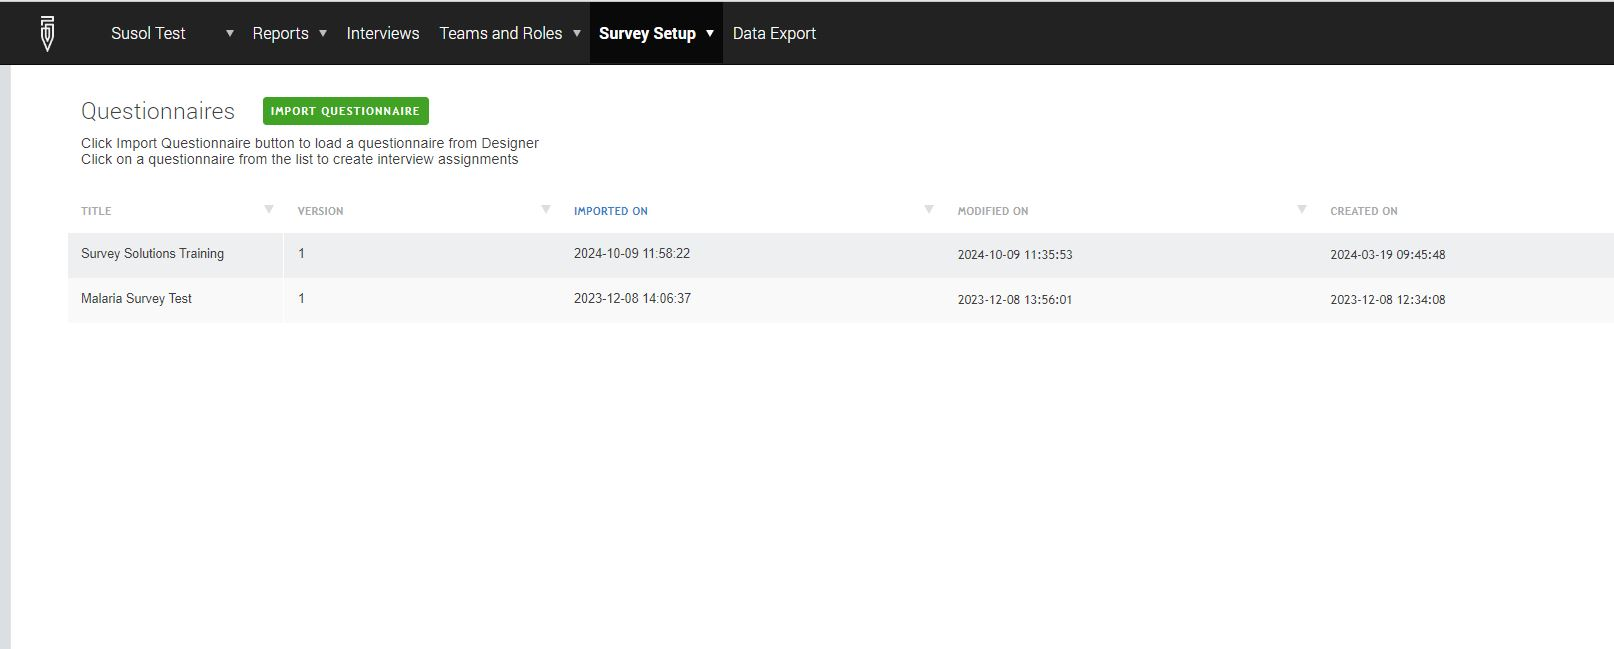
\includegraphics{images/login_susol.JPG}

  }

  \caption{Log in into the Survey Solution and pick the right workspace}

  \end{figure}%
\item
  \begin{figure}[H]

  {\centering 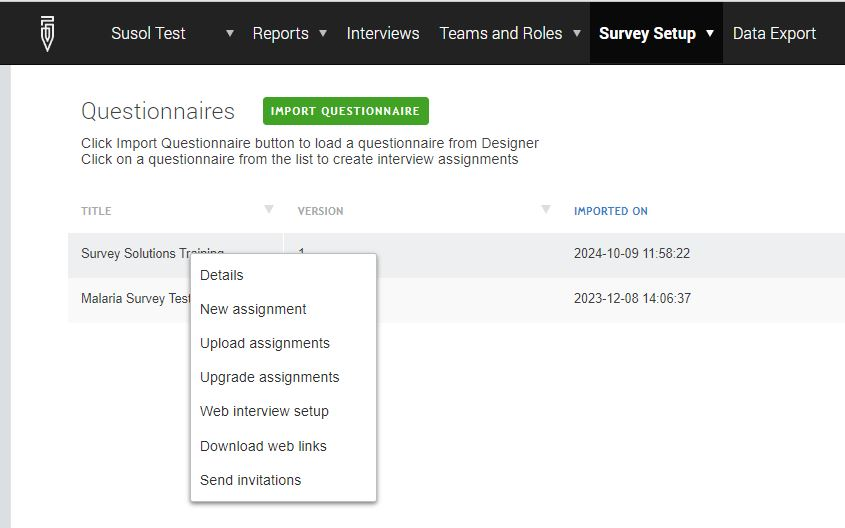
\includegraphics{images/click_quiz_details.JPG}

  }

  \caption{Click on desired questionnaire then select details}

  \end{figure}%
\item
  \begin{figure}[H]

  {\centering 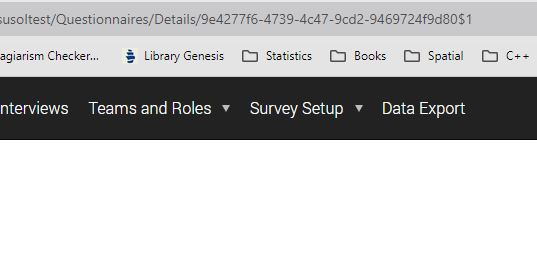
\includegraphics{images/quizid.JPG}

  }

  \caption{Locate the questionnaire at the address bar}

  \end{figure}%
\end{enumerate}

Between the \textbf{\emph{Details/}} and \textbf{\emph{\$}} sign is the
id.

\section{Download Script}\label{download-script}

The complete script to download data is given below:

\begin{Shaded}
\begin{Highlighting}[]
\CommentTok{\# Purpose: Download the trial dataset from the Survey Solutions server}
\CommentTok{\# Author: Moses Otieno}
\CommentTok{\# Date Created: 14 Oct 2024}
\CommentTok{\# Date Modified: 14 Oct 2024}

\CommentTok{\# {-}{-}{-}{-}{-} Modules required}

\ImportTok{import}\NormalTok{ requests}
\ImportTok{from}\NormalTok{ ssaw }\ImportTok{import}\NormalTok{ Client, ExportApi, QuestionnairesApi}
\ImportTok{from}\NormalTok{ ssaw }\ImportTok{import}\NormalTok{ models}
\ImportTok{from}\NormalTok{ time }\ImportTok{import}\NormalTok{ sleep}
\ImportTok{import}\NormalTok{ configparser}


\CommentTok{\# {-}{-}{-}{-} Read and get config values }

\NormalTok{config }\OperatorTok{=}\NormalTok{ configparser.ConfigParser()}
\NormalTok{config.read(}\StringTok{\textquotesingle{}config.ini\textquotesingle{}}\NormalTok{)}

\NormalTok{urls }\OperatorTok{=}\NormalTok{ [config[}\StringTok{\textquotesingle{}susol\textquotesingle{}}\NormalTok{][}\StringTok{\textquotesingle{}url\textquotesingle{}}\NormalTok{]]}

\NormalTok{survey\_test\_id }\OperatorTok{=}\NormalTok{ config[}\StringTok{\textquotesingle{}susol\textquotesingle{}}\NormalTok{][}\StringTok{\textquotesingle{}survey\_test\_id\textquotesingle{}}\NormalTok{]}
\NormalTok{mal\_id }\OperatorTok{=}\NormalTok{ config[}\StringTok{\textquotesingle{}susol\textquotesingle{}}\NormalTok{][}\StringTok{\textquotesingle{}mal\_id\textquotesingle{}}\NormalTok{]}

\CommentTok{\# {-}{-}{-}{-} Specify the questionnaires to download data from }

\NormalTok{questionnaires }\OperatorTok{=}\NormalTok{ \{}
    \StringTok{"survey\_test"}\NormalTok{: survey\_test\_id,}
    \StringTok{"malaria"}\NormalTok{: mal\_id}
\NormalTok{\}}


\CommentTok{\# {-}{-}{-}{-}{-} Define functions}

\KeywordTok{def}\NormalTok{ connect\_to\_internet(url}\OperatorTok{=}\StringTok{\textquotesingle{}http://www.google.com/\textquotesingle{}}\NormalTok{, timeout}\OperatorTok{=}\DecValTok{5}\NormalTok{):}
    \CommentTok{"""Check internet connectivity by pinging the given URL."""}
    \ControlFlowTok{try}\NormalTok{:}
\NormalTok{        \_ }\OperatorTok{=}\NormalTok{ requests.head(url, timeout}\OperatorTok{=}\NormalTok{timeout)}
        \ControlFlowTok{return} \VariableTok{True}
    \ControlFlowTok{except}\NormalTok{ requests.}\PreprocessorTok{ConnectionError}\NormalTok{:}
        \ControlFlowTok{return} \VariableTok{False}


\KeywordTok{def}\NormalTok{ connect\_to\_server():}
    \CommentTok{"""Attempt to connect to the Survey Solutions server via available URLs."""}
    \ControlFlowTok{for}\NormalTok{ url }\KeywordTok{in}\NormalTok{ urls:}
        \ControlFlowTok{if}\NormalTok{ connect\_to\_internet(url):}
            \BuiltInTok{print}\NormalTok{(}\SpecialStringTok{f\textquotesingle{}Connected to server: }\SpecialCharTok{\{}\NormalTok{url}\SpecialCharTok{\}}\SpecialStringTok{\textquotesingle{}}\NormalTok{)}
            \ControlFlowTok{return}\NormalTok{ url}
    \BuiltInTok{print}\NormalTok{(}\StringTok{"No connection to any server."}\NormalTok{)}
    \ControlFlowTok{return} \VariableTok{None}


\KeywordTok{def}\NormalTok{ get\_questionnaire\_versions(client, questionnaire\_id):}
    \CommentTok{"""Retrieve all versions of a questionnaire."""}
    \ControlFlowTok{return}\NormalTok{ [(q.}\BuiltInTok{id}\NormalTok{, q.version) }\ControlFlowTok{for}\NormalTok{ q }\KeywordTok{in}\NormalTok{ QuestionnairesApi(client).get\_list(questionnaire\_id}\OperatorTok{=}\NormalTok{questionnaire\_id)]}


\KeywordTok{def}\NormalTok{ download\_questionnaire\_data(client, qid, version, export\_path}\OperatorTok{=}\StringTok{\textquotesingle{}data\textquotesingle{}}\NormalTok{):}
    \CommentTok{"""Export and download questionnaire data in STATA format."""}
    \ControlFlowTok{try}\NormalTok{:}
\NormalTok{        export\_object }\OperatorTok{=}\NormalTok{ models.ExportJob(qid, export\_type}\OperatorTok{=}\StringTok{\textquotesingle{}STATA\textquotesingle{}}\NormalTok{)}
\NormalTok{        ExportApi(client).start(export\_object, wait}\OperatorTok{=}\VariableTok{True}\NormalTok{)}
\NormalTok{        ExportApi(client, workspace}\OperatorTok{=}\StringTok{"susoltest"}\NormalTok{).get(questionnaire\_identity}\OperatorTok{=}\NormalTok{qid, export\_type}\OperatorTok{=}\StringTok{\textquotesingle{}STATA\textquotesingle{}}\NormalTok{, show\_progress}\OperatorTok{=}\VariableTok{True}\NormalTok{, generate}\OperatorTok{=}\VariableTok{True}\NormalTok{, export\_path}\OperatorTok{=}\NormalTok{export\_path)}
        \BuiltInTok{print}\NormalTok{(}\SpecialStringTok{f\textquotesingle{}Successfully downloaded version: }\SpecialCharTok{\{}\NormalTok{version}\SpecialCharTok{\}}\SpecialStringTok{\textquotesingle{}}\NormalTok{)}
    \ControlFlowTok{except} \PreprocessorTok{Exception} \ImportTok{as}\NormalTok{ e:}
        \BuiltInTok{print}\NormalTok{(}\SpecialStringTok{f\textquotesingle{}Failed to download version: }\SpecialCharTok{\{}\NormalTok{version}\SpecialCharTok{\}}\SpecialStringTok{. Error: }\SpecialCharTok{\{}\NormalTok{e}\SpecialCharTok{\}}\SpecialStringTok{\textquotesingle{}}\NormalTok{)}


\KeywordTok{def}\NormalTok{ download\_all\_versions(client, qnrids, qnrversions):}
    \CommentTok{"""Loop through all versions of a questionnaire and download data."""}
    \ControlFlowTok{for}\NormalTok{ qnrid, version }\KeywordTok{in} \BuiltInTok{zip}\NormalTok{(qnrids, qnrversions):}
\NormalTok{        download\_questionnaire\_data(client, qnrid, version)}


\CommentTok{\# {-}{-}{-}{-}{-} Main execution logic}
\KeywordTok{def}\NormalTok{ main():}
    \CommentTok{\# Connect to the server and check internet connectivity}
\NormalTok{    server\_url }\OperatorTok{=} \VariableTok{None}
    \ControlFlowTok{for}\NormalTok{ attempt }\KeywordTok{in} \BuiltInTok{range}\NormalTok{(}\DecValTok{1}\NormalTok{, }\DecValTok{2}\NormalTok{):}
        \BuiltInTok{print}\NormalTok{(}\SpecialStringTok{f\textquotesingle{}Attempt }\SpecialCharTok{\{}\NormalTok{attempt}\SpecialCharTok{\}}\SpecialStringTok{ to connect...\textquotesingle{}}\NormalTok{)}
\NormalTok{        server\_url }\OperatorTok{=}\NormalTok{ connect\_to\_server()}
        \ControlFlowTok{if}\NormalTok{ server\_url:}
            \ControlFlowTok{break}
\NormalTok{        sleep(}\DecValTok{5}\NormalTok{)}
    \ControlFlowTok{if} \KeywordTok{not}\NormalTok{ server\_url:}
        \BuiltInTok{print}\NormalTok{(}\StringTok{"Failed to connect after 10 attempts."}\NormalTok{)}
        \ControlFlowTok{return}

    

    \CommentTok{\# Retrieve necessary configuration details}
\NormalTok{    api\_user }\OperatorTok{=}\NormalTok{ config[}\StringTok{\textquotesingle{}susol\textquotesingle{}}\NormalTok{][}\StringTok{\textquotesingle{}api\_user\textquotesingle{}}\NormalTok{]}
\NormalTok{    passwd }\OperatorTok{=}\NormalTok{ config[}\StringTok{\textquotesingle{}susol\textquotesingle{}}\NormalTok{][}\StringTok{\textquotesingle{}api\_password\textquotesingle{}}\NormalTok{]}
\NormalTok{    wkspace }\OperatorTok{=}\NormalTok{ config[}\StringTok{\textquotesingle{}susol\textquotesingle{}}\NormalTok{][}\StringTok{\textquotesingle{}workspace\textquotesingle{}}\NormalTok{]}
\NormalTok{    quizid }\OperatorTok{=}\NormalTok{ config[}\StringTok{\textquotesingle{}susol\textquotesingle{}}\NormalTok{][}\StringTok{\textquotesingle{}survey\_test\_id\textquotesingle{}}\NormalTok{]}

   \CommentTok{\# Initialize the Survey Solutions client}
   
\NormalTok{    client }\OperatorTok{=}\NormalTok{ Client(url}\OperatorTok{=}\NormalTok{server\_url, api\_user}\OperatorTok{=}\NormalTok{api\_user, api\_password}\OperatorTok{=}\NormalTok{passwd, workspace}\OperatorTok{=}\NormalTok{wkspace)}

    \CommentTok{\# Process each questionnaire}
    
    \ControlFlowTok{for}\NormalTok{ quizname, quizid }\KeywordTok{in}\NormalTok{ questionnaires.items():}
\NormalTok{        qnr\_data }\OperatorTok{=}\NormalTok{ get\_questionnaire\_versions(client, quizid)}
        \ControlFlowTok{if}\NormalTok{ qnr\_data:}
\NormalTok{            qnrids, qnrversions }\OperatorTok{=} \BuiltInTok{zip}\NormalTok{(}\OperatorTok{*}\NormalTok{qnr\_data)}
            \BuiltInTok{print}\NormalTok{(}\SpecialStringTok{f\textquotesingle{}The highest version of }\SpecialCharTok{\{}\NormalTok{quizname}\SpecialCharTok{\}}\SpecialStringTok{ is }\SpecialCharTok{\{}\BuiltInTok{max}\NormalTok{(qnrversions)}\SpecialCharTok{\}}\SpecialStringTok{. Downloading versions from }\SpecialCharTok{\{}\BuiltInTok{min}\NormalTok{(qnrversions)}\SpecialCharTok{\}}\SpecialStringTok{ to }\SpecialCharTok{\{}\BuiltInTok{max}\NormalTok{(qnrversions)}\SpecialCharTok{\}}\SpecialStringTok{.\textquotesingle{}}\NormalTok{)}
\NormalTok{            download\_all\_versions(client, qnrids, qnrversions)}
        \ControlFlowTok{else}\NormalTok{:}
            \BuiltInTok{print}\NormalTok{(}\SpecialStringTok{f\textquotesingle{}No versions found for }\SpecialCharTok{\{}\NormalTok{quizname}\SpecialCharTok{\}}\SpecialStringTok{.\textquotesingle{}}\NormalTok{)}

\ControlFlowTok{if} \VariableTok{\_\_name\_\_} \OperatorTok{==} \StringTok{"\_\_main\_\_"}\NormalTok{:}
\NormalTok{    main()}
\end{Highlighting}
\end{Shaded}

\subsection{Customizing Download
Script}\label{customizing-download-script}

You need to provide specific details in the script to download your
data:

\begin{enumerate}
\def\labelenumi{\arabic{enumi}.}
\item
  \textbf{config.ini}: Create a \texttt{config.ini} file with a section
  called \textbf{susol}. Include the required details:
  \texttt{api\ user}, \texttt{api\ password}, \texttt{url}, and
  \texttt{workspace}.
\item
  \textbf{Questionnaire}: Identify the IDs of the questionnaires you
  want to download and add them to the config file.
\item
  \textbf{export\_path}: Specify the download directory for the data.
  The script assumes there's a \textbf{data} directory in the same path;
  if not, create one or specify your desired directory.
\end{enumerate}

Once you have this information, you'll be able to download your data.

\subsection{Error Handling and
Debugging}\label{error-handling-and-debugging}

\begin{itemize}
\item
  If the script fails to connect, check your internet connection and the
  details in \texttt{config.ini}.
\item
  If you receive an ``Invalid Questionnaire ID'' error, verify that the
  IDs in the \texttt{questionnaires} dictionary are correct.
\item
  Monitor the output messages for any errors during the download
  process.
\end{itemize}

\subsection{Convention: Assigning One Workspace to One
Directory}\label{convention-assigning-one-workspace-to-one-directory}

In many data management and programming workflows, particularly when
dealing with multiple datasets, scripts, and configurations,
establishing a clear and consistent directory structure is essential for
maintaining organization and efficiency. I strongly advocate for the
convention of assigning one workspace to one directory. A workspace can
contain multiple questionnaires, so this script assumes that you will
work with each workspace separately.

\section{Summary}\label{summary}

Below is a summary of the steps you need to undertake in order to
download data from Survey Solutions server to your machine.

\begin{itemize}
\tightlist
\item
  \textbf{Create API User}: Ensure you have an API user created.
\item
  \textbf{Gather Information}: Collect the following:

  \begin{itemize}
  \item
    URL
  \item
    API username
  \item
    API password
  \item
    Workspace
  \item
    Questionnaire ID
  \end{itemize}
\item
  \textbf{Install \texttt{ssaw} Module}: Use Python to install the
  \texttt{ssaw} module.
\item
  \textbf{Create .ini Config File}: Store all necessary information for
  the Survey Solutions Server.
\item
  \textbf{Run the Script}: Execute the script to download the data!
\end{itemize}

To deepen your understanding in Python, I would recommend Automate the
Boring Stuff with Python\textsuperscript{2}. It is a highly praised book
that serves as an excellent introduction to programming for beginners,
particularly those looking to leverage Python for practical tasks. For
data management and analysis in Python, Python for data
analysis\textsuperscript{3} a good job.

\bookmarksetup{startatroot}

\chapter{Data Import}\label{data-import}

\section{Introduction}\label{introduction-2}

After downloading the data, the next step is to import it into your
programming environment for management. This section on data import is
essential because Survey Solutions stores the downloaded data in a
specific format. In our download script, we specified
\texttt{export\_type=\textquotesingle{}STATA\textquotesingle{}}, which I
prefer because STATA files include both variable labels and value
labels, eliminating the need to redefine them. Additionally, note that
the downloaded data is in a zipped format. If you have two versions of a
questionnaire, you'll receive two separate zipped files. There are two
ways you can import this data into R:

\begin{enumerate}
\def\labelenumi{\arabic{enumi}.}
\item
  \textbf{Manual Import}: Unzip each folder and then import the
  individual files into your programming environment.
\item
  \textbf{Automated Import}: Use a script to handle all the importing
  procedures, streamlining the process.
\end{enumerate}

Our focus will be the second one.

\section{Automated Import}\label{automated-import}

Using a \textbf{script to automate the import process} is generally more
efficient than manually unzipping and importing individual files. Here
are some reasons why:

\begin{enumerate}
\def\labelenumi{\arabic{enumi}.}
\item
  \textbf{Time-Saving}: A script can process multiple files in a single
  run, eliminating the need for repetitive manual actions.
\item
  \textbf{Reduced Errors}: Automating the process minimizes the risk of
  human error that can occur during manual imports, such as skipping
  files or importing them incorrectly.
\item
  \textbf{Consistency}: A script ensures that the same import process is
  followed every time, leading to consistent results.
\item
  \textbf{Scalability}: If the number of files or datasets increases, a
  script can easily accommodate the additional data without requiring
  more manual effort.
\item
  \textbf{Easy Adjustments}: If changes are needed (e.g., modifying file
  paths or import settings), you can update the script instead of
  repeating the manual steps.
\item
  \textbf{Adaptability}: you can use the same script for different
  projects with minimal changes.
\end{enumerate}

\section{Survey Solutions Data
Structure}\label{survey-solutions-data-structure}

Before diving into data importation, it's crucial to understand the
structure of the zipped directory and its contents from Survey
Solutions. This knowledge will help you navigate the files efficiently
and ensure that you are importing the correct data. The naming
convention is
\textbf{\emph{questionnaire-name\_versionnumber\_Exporttype\_All.zip.}}
Example \emph{ssolutions\_training\_1\_STATA\_All.zip.}

\begin{figure}[H]

{\centering 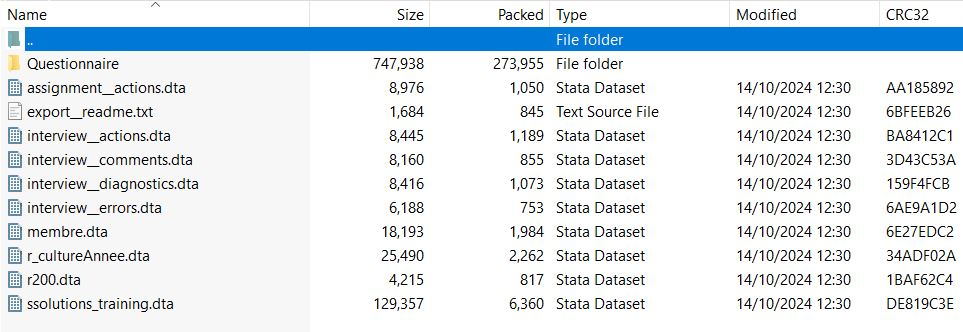
\includegraphics{images/data_pieces.JPG}

}

\caption{Contents of zipped directory}

\end{figure}%

The contents include the data and metadata:

\subsection{Metadata Files}\label{metadata-files}

These files provide additional context about the data. They include:

\begin{itemize}
\item
  assignment\_actions
\item
  interview\_actions
\item
  interview\_comments
\item
  interview\_diagnostics
\item
  interview\_errors
\item
  Questionnaire: A directory containing the questionnaire
\end{itemize}

\subsection{Data Files}\label{data-files}

The data files are the core components of the downloaded dataset from
Survey Solutions. Here's a closer look at their significance and
structure:

\begin{enumerate}
\def\labelenumi{\arabic{enumi}.}
\item
  \textbf{Main Questionnaire File}:

  \begin{itemize}
  \tightlist
  \item
    This file is named after the questionnaire itself and serves as the
    primary dataset containing the survey responses. The questionnaire
    variable is crucial here, as it uniquely identifies the survey you
    conducted. This unique name allows you to easily reference and
    manage the data throughout your analysis. In this context it is
    \textbf{\emph{ssolutions\_training}}
  \end{itemize}
\item
  \textbf{Roster Datasets}:

  \begin{itemize}
  \item
    In addition to the main questionnaire file, there may be several
    additional files that contain data from rosters. Rosters are used in
    surveys to collect information on groups of similar items or
    respondents (e.g., household members, patients, etc.).
  \item
    Each roster file contains responses related to specific sections of
    the questionnaire and may include variables corresponding to
    individual roster entries.
  \end{itemize}
\end{enumerate}

\section{Import Data in R}\label{import-data-in-r}

Now that you understand the data structure and the contents of the
zipped files from Survey Solutions, let's dive into the process of
importing this data into R. Importing data correctly is crucial for
effective management and analysis.

The packages for use include:

\begin{Shaded}
\begin{Highlighting}[]
\FunctionTok{library}\NormalTok{(tidyverse)          }\CommentTok{\# Data management}
\FunctionTok{library}\NormalTok{(haven)              }\CommentTok{\# Import the stata files}
\end{Highlighting}
\end{Shaded}

The body of the code is below:

\begin{Shaded}
\begin{Highlighting}[]
\CommentTok{\# | include: false}

\CommentTok{\#{-}{-}{-}{-} List all the zip files. These are different versions of the questionnaire}

\NormalTok{all\_zips }\OtherTok{\textless{}{-}} \FunctionTok{list.files}\NormalTok{(}\StringTok{"data"}\NormalTok{, }\AttributeTok{pattern =} \StringTok{"ssolutions\_training.*.zip"}\NormalTok{,}
                       \AttributeTok{full.names =}\NormalTok{ T)}


\CommentTok{\# {-}{-}{-}{-} Download main questionnaire}

\NormalTok{all\_ssolutions\_training }\OtherTok{\textless{}{-}} \FunctionTok{vector}\NormalTok{(}\StringTok{"list"}\NormalTok{)}

\ControlFlowTok{for}\NormalTok{ (zipfile }\ControlFlowTok{in}\NormalTok{ all\_zips)\{}

\NormalTok{  qversion }\OtherTok{\textless{}{-}} \FunctionTok{str\_extract}\NormalTok{(zipfile, }\StringTok{"\_}\SpecialCharTok{\textbackslash{}\textbackslash{}}\StringTok{d+\_STATA\_"}\NormalTok{)}
\NormalTok{  qversion }\OtherTok{\textless{}{-}} \FunctionTok{parse\_number}\NormalTok{(qversion)}


  \FunctionTok{unzip}\NormalTok{(zipfile, }\AttributeTok{files =} \FunctionTok{c}\NormalTok{(}\StringTok{"ssolutions\_training.dta"}\NormalTok{),}
        \AttributeTok{exdir =} \StringTok{"data"}\NormalTok{)}


\NormalTok{  all\_ssolutions\_training[[zipfile]] }\OtherTok{\textless{}{-}} \FunctionTok{read\_dta}\NormalTok{(}\StringTok{"data/ssolutions\_training.dta"}\NormalTok{) }\SpecialCharTok{|\textgreater{}}
    \FunctionTok{mutate}\NormalTok{(}\AttributeTok{quiz\_version =}\NormalTok{ qversion)}
\NormalTok{\}}



\NormalTok{ssolutions\_training }\OtherTok{\textless{}{-}}\NormalTok{ all\_ssolutions\_training }\SpecialCharTok{|\textgreater{}} 
  \FunctionTok{map}\NormalTok{(bind\_rows, }\AttributeTok{.progress =} \ConstantTok{TRUE}\NormalTok{) }\SpecialCharTok{|\textgreater{}}  
  \FunctionTok{list\_rbind}\NormalTok{() }


\CommentTok{\# {-}{-}{-}{-} Save the main questionnaire}

\FunctionTok{write\_rds}\NormalTok{(ssolutions\_training, }\StringTok{"data/ssolutions\_training\_main.rds"}\NormalTok{)}


\CommentTok{\# {-}{-}{-}{-} Download the rosters}

\NormalTok{all\_membre }\OtherTok{\textless{}{-}} \FunctionTok{vector}\NormalTok{(}\StringTok{"list"}\NormalTok{)}
\NormalTok{all\_cultureanne }\OtherTok{\textless{}{-}} \FunctionTok{vector}\NormalTok{(}\StringTok{"list"}\NormalTok{)}
\NormalTok{all\_r200 }\OtherTok{\textless{}{-}} \FunctionTok{vector}\NormalTok{(}\StringTok{"list"}\NormalTok{)}


\ControlFlowTok{for}\NormalTok{ (zipfile }\ControlFlowTok{in}\NormalTok{ all\_zips)\{}

\NormalTok{  qversion }\OtherTok{\textless{}{-}} \FunctionTok{str\_extract}\NormalTok{(zipfile, }\StringTok{"\_}\SpecialCharTok{\textbackslash{}\textbackslash{}}\StringTok{d+\_STATA\_"}\NormalTok{)}
\NormalTok{  qversion }\OtherTok{\textless{}{-}} \FunctionTok{parse\_number}\NormalTok{(qversion)}


  \FunctionTok{unzip}\NormalTok{(zipfile, }\AttributeTok{files =} \FunctionTok{c}\NormalTok{(}\StringTok{"membre.dta"}\NormalTok{, }\StringTok{"r\_cultureAnnee.dta"}\NormalTok{, }\StringTok{"r200.dta"}\NormalTok{),}
        \AttributeTok{exdir =} \StringTok{"data"}\NormalTok{)}


\NormalTok{  all\_membre[[zipfile]] }\OtherTok{\textless{}{-}} \FunctionTok{read\_dta}\NormalTok{(}\StringTok{"data/membre.dta"}\NormalTok{) }\SpecialCharTok{|\textgreater{}}
    \FunctionTok{mutate}\NormalTok{(}\AttributeTok{quiz\_version =}\NormalTok{ qversion)}
  
\NormalTok{  all\_cultureanne[[zipfile]] }\OtherTok{\textless{}{-}} \FunctionTok{read\_dta}\NormalTok{(}\StringTok{"data/r\_cultureAnnee.dta"}\NormalTok{) }\SpecialCharTok{|\textgreater{}}
    \FunctionTok{mutate}\NormalTok{(}\AttributeTok{quiz\_version =}\NormalTok{ qversion)}
  
  
\NormalTok{  all\_r200[[zipfile]] }\OtherTok{\textless{}{-}} \FunctionTok{read\_dta}\NormalTok{(}\StringTok{"data/r200.dta"}\NormalTok{) }\SpecialCharTok{|\textgreater{}}
    \FunctionTok{mutate}\NormalTok{(}\AttributeTok{quiz\_version =}\NormalTok{ qversion)}
  
\NormalTok{\}}


\NormalTok{membre }\OtherTok{\textless{}{-}}\NormalTok{ all\_membre }\SpecialCharTok{|\textgreater{}} 
  \FunctionTok{map}\NormalTok{(bind\_rows, }\AttributeTok{.progress =} \ConstantTok{TRUE}\NormalTok{) }\SpecialCharTok{|\textgreater{}}  
  \FunctionTok{list\_rbind}\NormalTok{() }


\NormalTok{cultureanne }\OtherTok{\textless{}{-}}\NormalTok{ all\_cultureanne }\SpecialCharTok{|\textgreater{}} 
  \FunctionTok{map}\NormalTok{(bind\_rows, }\AttributeTok{.progress =} \ConstantTok{TRUE}\NormalTok{) }\SpecialCharTok{|\textgreater{}}  
  \FunctionTok{list\_rbind}\NormalTok{() }

\NormalTok{r200 }\OtherTok{\textless{}{-}}\NormalTok{ all\_r200 }\SpecialCharTok{|\textgreater{}} 
  \FunctionTok{map}\NormalTok{(bind\_rows, }\AttributeTok{.progress =} \ConstantTok{TRUE}\NormalTok{) }\SpecialCharTok{|\textgreater{}}  
  \FunctionTok{list\_rbind}\NormalTok{() }
\end{Highlighting}
\end{Shaded}

\subsection{Full Script}\label{full-script}

\begin{Shaded}
\begin{Highlighting}[]
\FunctionTok{library}\NormalTok{(tidyverse)          }\CommentTok{\# Data management}
\FunctionTok{library}\NormalTok{(haven)              }\CommentTok{\# Import the stata files}

\CommentTok{\#{-}{-}{-}{-} List all the zip files. These are different versions of the questionnaire}

\NormalTok{all\_zips }\OtherTok{\textless{}{-}} \FunctionTok{list.files}\NormalTok{(}\StringTok{"data"}\NormalTok{, }\AttributeTok{pattern =} \StringTok{"ssolutions\_training.*.zip"}\NormalTok{,}
                       \AttributeTok{full.names =}\NormalTok{ T)}


\CommentTok{\# {-}{-}{-}{-} Download main questionnaire}

\NormalTok{all\_ssolutions\_training }\OtherTok{\textless{}{-}} \FunctionTok{vector}\NormalTok{(}\StringTok{"list"}\NormalTok{)}

\ControlFlowTok{for}\NormalTok{ (zipfile }\ControlFlowTok{in}\NormalTok{ all\_zips)\{}

\NormalTok{  qversion }\OtherTok{\textless{}{-}} \FunctionTok{str\_extract}\NormalTok{(zipfile, }\StringTok{"\_}\SpecialCharTok{\textbackslash{}\textbackslash{}}\StringTok{d+\_STATA\_"}\NormalTok{)}
\NormalTok{  qversion }\OtherTok{\textless{}{-}} \FunctionTok{parse\_number}\NormalTok{(qversion)}


  \FunctionTok{unzip}\NormalTok{(zipfile, }\AttributeTok{files =} \FunctionTok{c}\NormalTok{(}\StringTok{"ssolutions\_training.dta"}\NormalTok{),}
        \AttributeTok{exdir =} \StringTok{"data"}\NormalTok{)}


\NormalTok{  all\_ssolutions\_training[[zipfile]] }\OtherTok{\textless{}{-}} \FunctionTok{read\_dta}\NormalTok{(}\StringTok{"data/ssolutions\_training.dta"}\NormalTok{) }\SpecialCharTok{|\textgreater{}}
    \FunctionTok{mutate}\NormalTok{(}\AttributeTok{quiz\_version =}\NormalTok{ qversion)}
\NormalTok{\}}



\NormalTok{ssolutions\_training }\OtherTok{\textless{}{-}}\NormalTok{ all\_ssolutions\_training }\SpecialCharTok{|\textgreater{}} 
  \FunctionTok{map}\NormalTok{(bind\_rows, }\AttributeTok{.progress =} \ConstantTok{TRUE}\NormalTok{) }\SpecialCharTok{|\textgreater{}}  
  \FunctionTok{list\_rbind}\NormalTok{() }

\CommentTok{\# {-}{-}{-}{-} Save the main questionnaire}

\FunctionTok{write\_rds}\NormalTok{(ssolutions\_training, }\StringTok{"ssolutions\_training\_main.rds"}\NormalTok{)}


\CommentTok{\# {-}{-}{-}{-} Download the rosters}

\NormalTok{all\_membre }\OtherTok{\textless{}{-}} \FunctionTok{vector}\NormalTok{(}\StringTok{"list"}\NormalTok{)}
\NormalTok{all\_cultureanne }\OtherTok{\textless{}{-}} \FunctionTok{vector}\NormalTok{(}\StringTok{"list"}\NormalTok{)}
\NormalTok{all\_r200 }\OtherTok{\textless{}{-}} \FunctionTok{vector}\NormalTok{(}\StringTok{"list"}\NormalTok{)}


\ControlFlowTok{for}\NormalTok{ (zipfile }\ControlFlowTok{in}\NormalTok{ all\_zips)\{}

\NormalTok{  qversion }\OtherTok{\textless{}{-}} \FunctionTok{str\_extract}\NormalTok{(zipfile, }\StringTok{"\_}\SpecialCharTok{\textbackslash{}\textbackslash{}}\StringTok{d+\_STATA\_"}\NormalTok{)}
\NormalTok{  qversion }\OtherTok{\textless{}{-}} \FunctionTok{parse\_number}\NormalTok{(qversion)}


  \FunctionTok{unzip}\NormalTok{(zipfile, }\AttributeTok{files =} \FunctionTok{c}\NormalTok{(}\StringTok{"membre.dta"}\NormalTok{, }\StringTok{"r\_cultureAnnee.dta"}\NormalTok{, }\StringTok{"r200.dta"}\NormalTok{),}
        \AttributeTok{exdir =} \StringTok{"data"}\NormalTok{)}


\NormalTok{  all\_membre[[zipfile]] }\OtherTok{\textless{}{-}} \FunctionTok{read\_dta}\NormalTok{(}\StringTok{"data/membre.dta"}\NormalTok{) }\SpecialCharTok{|\textgreater{}}
    \FunctionTok{mutate}\NormalTok{(}\AttributeTok{quiz\_version =}\NormalTok{ qversion)}
  
\NormalTok{  all\_cultureanne[[zipfile]] }\OtherTok{\textless{}{-}} \FunctionTok{read\_dta}\NormalTok{(}\StringTok{"data/r\_cultureAnnee.dta"}\NormalTok{) }\SpecialCharTok{|\textgreater{}}
    \FunctionTok{mutate}\NormalTok{(}\AttributeTok{quiz\_version =}\NormalTok{ qversion)}
  
  
\NormalTok{  all\_r200[[zipfile]] }\OtherTok{\textless{}{-}} \FunctionTok{read\_dta}\NormalTok{(}\StringTok{"data/r200.dta"}\NormalTok{) }\SpecialCharTok{|\textgreater{}}
    \FunctionTok{mutate}\NormalTok{(}\AttributeTok{quiz\_version =}\NormalTok{ qversion)}
  
\NormalTok{\}}


\NormalTok{membre }\OtherTok{\textless{}{-}}\NormalTok{ all\_membre }\SpecialCharTok{|\textgreater{}} 
  \FunctionTok{map}\NormalTok{(bind\_rows, }\AttributeTok{.progress =} \ConstantTok{TRUE}\NormalTok{) }\SpecialCharTok{|\textgreater{}}  
  \FunctionTok{list\_rbind}\NormalTok{() }


\NormalTok{cultureanne }\OtherTok{\textless{}{-}}\NormalTok{ all\_cultureanne }\SpecialCharTok{|\textgreater{}} 
  \FunctionTok{map}\NormalTok{(bind\_rows, }\AttributeTok{.progress =} \ConstantTok{TRUE}\NormalTok{) }\SpecialCharTok{|\textgreater{}}  
  \FunctionTok{list\_rbind}\NormalTok{() }

\NormalTok{r200 }\OtherTok{\textless{}{-}}\NormalTok{ all\_r200 }\SpecialCharTok{|\textgreater{}} 
  \FunctionTok{map}\NormalTok{(bind\_rows, }\AttributeTok{.progress =} \ConstantTok{TRUE}\NormalTok{) }\SpecialCharTok{|\textgreater{}}  
  \FunctionTok{list\_rbind}\NormalTok{() }

\FunctionTok{write\_rds}\NormalTok{(membre, }\StringTok{"data/membre.rds"}\NormalTok{)}
\FunctionTok{write\_rds}\NormalTok{(cultureanne, }\StringTok{"data/cultureanne.rds"}\NormalTok{)}
\FunctionTok{write\_rds}\NormalTok{(r200, }\StringTok{"data/r200.rds"}\NormalTok{)}
\end{Highlighting}
\end{Shaded}

\subsection{Optimised Code}\label{optimised-code}

\begin{Shaded}
\begin{Highlighting}[]
\FunctionTok{library}\NormalTok{(tidyverse)          }\CommentTok{\# Data management}
\FunctionTok{library}\NormalTok{(haven)              }\CommentTok{\# Import the Stata files}

\CommentTok{\# {-}{-}{-}{-} List all the zip files. These are different versions of the questionnaire}
\NormalTok{all\_zips }\OtherTok{\textless{}{-}} \FunctionTok{list.files}\NormalTok{(}\StringTok{"data"}\NormalTok{, }\AttributeTok{pattern =} \StringTok{"ssolutions\_training.*.zip"}\NormalTok{, }
                       \AttributeTok{full.names =} \ConstantTok{TRUE}\NormalTok{)}

\CommentTok{\# {-}{-}{-}{-} Function to extract and read data}
\NormalTok{read\_data\_from\_zip }\OtherTok{\textless{}{-}} \ControlFlowTok{function}\NormalTok{(zipfile, file\_name, qversion) \{}
  \FunctionTok{unzip}\NormalTok{(zipfile, }\AttributeTok{files =}\NormalTok{ file\_name, }\AttributeTok{exdir =} \StringTok{"data"}\NormalTok{)}
  \FunctionTok{read\_dta}\NormalTok{(}\FunctionTok{file.path}\NormalTok{(}\StringTok{"data"}\NormalTok{, file\_name)) }\SpecialCharTok{\%\textgreater{}\%} \FunctionTok{mutate}\NormalTok{(}\AttributeTok{quiz\_version =}\NormalTok{ qversion)}
\NormalTok{\}}

\CommentTok{\# {-}{-}{-}{-} Download main questionnaire}
\NormalTok{all\_ssolutions\_training }\OtherTok{\textless{}{-}} \FunctionTok{map}\NormalTok{(all\_zips, }\ControlFlowTok{function}\NormalTok{(zipfile) \{}
\NormalTok{  qversion }\OtherTok{\textless{}{-}} \FunctionTok{parse\_number}\NormalTok{(}\FunctionTok{str\_extract}\NormalTok{(zipfile, }\StringTok{"\_}\SpecialCharTok{\textbackslash{}\textbackslash{}}\StringTok{d+\_STATA\_"}\NormalTok{))}
  \FunctionTok{read\_data\_from\_zip}\NormalTok{(zipfile, }\StringTok{"ssolutions\_training.dta"}\NormalTok{, qversion)}
\NormalTok{\})}

\NormalTok{ssolutions\_training }\OtherTok{\textless{}{-}} \FunctionTok{bind\_rows}\NormalTok{(all\_ssolutions\_training, }\AttributeTok{.id =} \StringTok{"source"}\NormalTok{)  }\CommentTok{\# Add a source column if needed}

\CommentTok{\# {-}{-}{-}{-} Save the main questionnaire}
\FunctionTok{write\_rds}\NormalTok{(ssolutions\_training, }\StringTok{"data/ssolutions\_training\_main.rds"}\NormalTok{)}

\CommentTok{\# {-}{-}{-}{-} Download the rosters}
\NormalTok{all\_rosters }\OtherTok{\textless{}{-}} \FunctionTok{map}\NormalTok{(all\_zips, }\ControlFlowTok{function}\NormalTok{(zipfile) \{}
\NormalTok{  qversion }\OtherTok{\textless{}{-}} \FunctionTok{parse\_number}\NormalTok{(}\FunctionTok{str\_extract}\NormalTok{(zipfile, }\StringTok{"\_}\SpecialCharTok{\textbackslash{}\textbackslash{}}\StringTok{d+\_STATA\_"}\NormalTok{))}
  
  \CommentTok{\# Read all roster files into a list}
\NormalTok{  roster\_files }\OtherTok{\textless{}{-}} \FunctionTok{c}\NormalTok{(}\StringTok{"membre.dta"}\NormalTok{, }\StringTok{"r\_cultureAnnee.dta"}\NormalTok{, }\StringTok{"r200.dta"}\NormalTok{)}
  \FunctionTok{map}\NormalTok{(roster\_files, }\SpecialCharTok{\textasciitilde{}} \FunctionTok{read\_data\_from\_zip}\NormalTok{(zipfile, ., qversion))}
\NormalTok{\})}

\CommentTok{\# {-}{-}{-}{-} Combine roster data}
\NormalTok{membre }\OtherTok{\textless{}{-}} \FunctionTok{bind\_rows}\NormalTok{(}\FunctionTok{map}\NormalTok{(all\_rosters, }\StringTok{\textasciigrave{}}\AttributeTok{[[}\StringTok{\textasciigrave{}}\NormalTok{, }\DecValTok{1}\NormalTok{), }\AttributeTok{.id =} \StringTok{"source"}\NormalTok{)  }\CommentTok{\# First roster: membre}
\NormalTok{cultureanne }\OtherTok{\textless{}{-}} \FunctionTok{bind\_rows}\NormalTok{(}\FunctionTok{map}\NormalTok{(all\_rosters, }\StringTok{\textasciigrave{}}\AttributeTok{[[}\StringTok{\textasciigrave{}}\NormalTok{, }\DecValTok{2}\NormalTok{), }\AttributeTok{.id =} \StringTok{"source"}\NormalTok{)  }\CommentTok{\# Second roster: r\_cultureAnnee}
\NormalTok{r200 }\OtherTok{\textless{}{-}} \FunctionTok{bind\_rows}\NormalTok{(}\FunctionTok{map}\NormalTok{(all\_rosters, }\StringTok{\textasciigrave{}}\AttributeTok{[[}\StringTok{\textasciigrave{}}\NormalTok{, }\DecValTok{3}\NormalTok{), }\AttributeTok{.id =} \StringTok{"source"}\NormalTok{)  }\CommentTok{\# Third roster: r200}


\FunctionTok{write\_rds}\NormalTok{(membre, }\StringTok{"data/membre.rds"}\NormalTok{)}
\FunctionTok{write\_rds}\NormalTok{(cultureanne, }\StringTok{"data/cultureanne.rds"}\NormalTok{)}
\FunctionTok{write\_rds}\NormalTok{(r200, }\StringTok{"data/r200.rds"}\NormalTok{)}
\end{Highlighting}
\end{Shaded}

\bookmarksetup{startatroot}

\chapter{Data Cleaning}\label{data-cleaning}

\section{Introduction}\label{introduction-3}

Data cleaning is a vital step in data analysis, ensuring accuracy and
consistency in your dataset. While there isn't a one-size-fits-all
template, each dataset presents unique challenges that require
context-specific solutions. A thorough understanding of the study design
is key to effective data cleaning. For instance, cross-sectional studies
should have unique participant records, whereas longitudinal studies
involve repeated measures.

Another crucial detail is the \textbf{unit of analysis}. For example, in
datasets involving households and their members, it's essential to
understand how households and participants are uniquely identified to
ensure accurate data handling.

\subsection{Primary Key}\label{primary-key}

A \textbf{primary key} is a unique identifier for each record in a
dataset, ensuring that no two rows are identical. It is crucial for
maintaining data integrity, especially when dealing with relational
databases or complex datasets. The primary key allows you to retrieve,
update, or relate specific records without ambiguity.

In a dataset involving households and members, for example:

\begin{itemize}
\item
  \textbf{Household ID} might be the primary key for identifying
  households.
\item
  \textbf{Member ID} (within a household) could serve as a secondary key
  to uniquely identify individuals in relation to the household.
\end{itemize}

The primary key is essential for linking related tables (e.g., household
and member tables) and avoiding data duplication or inconsistencies. The
study design should have a mechanism of uniquely identifying the records
in a dataset.

\subsection{Survey Solutions Primary
Key}\label{survey-solutions-primary-key}

In \textbf{Survey Solutions}, linking the main questionnaire dataset
with roster datasets is done through two key variables:

\begin{enumerate}
\def\labelenumi{\arabic{enumi}.}
\item
  \textbf{interview\_key}: This is a user-friendly identifier used to
  uniquely reference interviews. It can be helpful when referencing or
  reviewing specific interviews during data collection or management.
\item
  \textbf{interview\_id}: This is a unique identifier generated by the
  system for each interview. It serves as a reliable key to link
  datasets, including the main questionnaire and any associated rosters,
  ensuring consistency and accuracy when combining data across various
  sections of the study.
\end{enumerate}

These variables play a critical role in maintaining the integrity of
data across the different components of the survey.

\section{Common Data Cleaning
Process}\label{common-data-cleaning-process}

\begin{Shaded}
\begin{Highlighting}[]
\FunctionTok{library}\NormalTok{(tidyverse)}
\FunctionTok{library}\NormalTok{(janitor)}
\FunctionTok{library}\NormalTok{(haven)}
\end{Highlighting}
\end{Shaded}

\subsection{Cleaning Column Names}\label{cleaning-column-names}

\begin{Shaded}
\begin{Highlighting}[]
\NormalTok{sstraining\_main }\OtherTok{\textless{}{-}} \FunctionTok{read\_rds}\NormalTok{(}\StringTok{"data/ssolutions\_training\_main.rds"}\NormalTok{)}



\NormalTok{sstraining\_main }\OtherTok{\textless{}{-}}\NormalTok{ sstraining\_main }\SpecialCharTok{|\textgreater{}} 
  \FunctionTok{clean\_names}\NormalTok{()}


\NormalTok{members }\OtherTok{\textless{}{-}} \FunctionTok{read\_rds}\NormalTok{(}\StringTok{"data/membre.rds"}\NormalTok{)}

\NormalTok{members }\OtherTok{\textless{}{-}}\NormalTok{ members }\SpecialCharTok{|\textgreater{}} 
  \FunctionTok{clean\_names}\NormalTok{()}
\end{Highlighting}
\end{Shaded}

\subsection{Check Duplicates}\label{check-duplicates}

\begin{Shaded}
\begin{Highlighting}[]
\NormalTok{dups\_ssmain }\OtherTok{\textless{}{-}}\NormalTok{ sstraining\_main }\SpecialCharTok{|\textgreater{}} 
  \FunctionTok{get\_dupes}\NormalTok{(idhh)}
\end{Highlighting}
\end{Shaded}

\subsection{Handle Missing Values}\label{handle-missing-values}

\begin{Shaded}
\begin{Highlighting}[]
\FunctionTok{library}\NormalTok{(naniar) }
\NormalTok{generate\_missing\_report }\OtherTok{\textless{}{-}} \ControlFlowTok{function}\NormalTok{(data) \{}
\NormalTok{  missing\_report }\OtherTok{\textless{}{-}} \FunctionTok{miss\_var\_summary}\NormalTok{(data, }\AttributeTok{order =} \ConstantTok{TRUE}\NormalTok{,}
                                     \AttributeTok{add\_cumsum =} \ConstantTok{TRUE}\NormalTok{)  }\SpecialCharTok{|\textgreater{}} 
    \FunctionTok{filter}\NormalTok{(n\_miss }\SpecialCharTok{!=} \DecValTok{0}\NormalTok{) }\SpecialCharTok{\%\textgreater{}\%}
\NormalTok{    dplyr}\SpecialCharTok{::}\FunctionTok{select}\NormalTok{(variable, pct\_miss, n\_miss)  }\SpecialCharTok{|\textgreater{}} 
    \FunctionTok{mutate}\NormalTok{(}\AttributeTok{pct\_miss =} \FunctionTok{round}\NormalTok{(pct\_miss, }\DecValTok{1}\NormalTok{)) }\SpecialCharTok{|\textgreater{}} 
    \FunctionTok{filter}\NormalTok{(pct\_miss }\SpecialCharTok{\textgreater{}} \DecValTok{0}\NormalTok{) }\SpecialCharTok{|\textgreater{}} 
    \FunctionTok{rename}\NormalTok{(}\AttributeTok{percentage\_missing =}\NormalTok{ pct\_miss)}
  
\NormalTok{  missing\_report}
  
\NormalTok{\}}


\FunctionTok{generate\_missing\_report}\NormalTok{(sstraining\_main)}
\end{Highlighting}
\end{Shaded}

\begin{verbatim}
# A tibble: 17 x 3
   variable        percentage_missing n_miss
   <chr>                        <dbl>  <int>
 1 q_aepotravail_1                100      1
 2 q_aepotravail_2                100      1
 3 q_aepotravail_3                100      1
 4 q_aepotravail_4                100      1
 5 q_aepotravail_9                100      1
 6 qd24a_1                        100      1
 7 qd24a_2                        100      1
 8 qd24a_3                        100      1
 9 qd25                           100      1
10 qd26                           100      1
11 qd27                           100      1
12 qd28                           100      1
13 qd29                           100      1
14 qd30                           100      1
15 qd31                           100      1
16 qd32                           100      1
17 qd32a                          100      1
\end{verbatim}

\begin{Shaded}
\begin{Highlighting}[]
\NormalTok{sstraining\_main }\OtherTok{\textless{}{-}}\NormalTok{ sstraining\_main }\SpecialCharTok{|\textgreater{}} 
  \FunctionTok{remove\_empty}\NormalTok{(}\AttributeTok{which =} \FunctionTok{c}\NormalTok{(}\StringTok{"rows"}\NormalTok{, }\StringTok{"cols"}\NormalTok{))}
\end{Highlighting}
\end{Shaded}

\subsection{Type Casting}\label{type-casting}

This process involves transforming data from one type to another, such
as converting a string to a number, or an integer to a floating-point
number, depending on the requirements of the operation.

\begin{Shaded}
\begin{Highlighting}[]
\NormalTok{sstraining\_main }\OtherTok{\textless{}{-}}\NormalTok{ sstraining\_main }\SpecialCharTok{|\textgreater{}} 
  \FunctionTok{mutate}\NormalTok{(}\FunctionTok{across}\NormalTok{(}\FunctionTok{where}\NormalTok{(is.labelled), as\_factor))}
\end{Highlighting}
\end{Shaded}

I usually convert labeled types to factors which are useful in further
analysis.

\subsection{Labeling Variables}\label{labeling-variables}

One of the significant advantages of using \textbf{Survey Solutions} is
the ability to label variables at the time of questionnaire design. This
feature ensures that each variable in your survey is clearly identified
with a meaningful label, which simplifies data management and analysis
later on.

However you may want to manually label the variables.

\begin{Shaded}
\begin{Highlighting}[]
\FunctionTok{attr}\NormalTok{(sstraining\_main[[}\StringTok{\textquotesingle{}qa03\textquotesingle{}}\NormalTok{]], }\StringTok{\textquotesingle{}label\textquotesingle{}}\NormalTok{) }\OtherTok{\textless{}{-}} \StringTok{"Pay non{-}family members to work on your fields"}

\FunctionTok{write\_rds}\NormalTok{(sstraining\_main, }\StringTok{"data/sstraining\_main\_clean.rds"}\NormalTok{)}
\end{Highlighting}
\end{Shaded}

\section{Summary}\label{summary-1}

Data cleaning is inherently context-specific, meaning there is no
universal template that fits all scenarios. To effectively clean your
data, it is essential to thoroughly understand the study design,
objectives, and other relevant factors. This knowledge allows for a
tailored approach that addresses the unique requirements of the dataset
and the goals of the analysis.

To master R, I recommend \textbf{R for Data Science}\textsuperscript{4}.
This book introduces the tidyverse and focuses on data manipulation,
visualization, and analysis through practical examples and exercises.
Its clear explanations and structured approach make it suitable for both
beginners and those looking to enhance their skills. Whether you're
starting out or aiming to deepen your expertise, this book is a reliable
guide for your data science journey

\bookmarksetup{startatroot}

\chapter{Report Generation}\label{report-generation}

\section{Introduction}\label{introduction-4}

The ultimate objective of any data preprocessing effort is to generate
useful data output. Whether it's calculating summary statistics of key
variables, tracking data collection progress, building dashboards with
actionable insights, developing complex models, or creating other data
products, reporting is essential to communicate findings effectively.

Generating real-time progress reports during data collection is
especially important. This allows you to catch potential issues early
on, such as:

\begin{itemize}
\item
  Missed skip logic
\item
  Incorrect validation rules
\item
  Other data-related inconsistencies
\end{itemize}

These insights enable immediate corrective actions, ensuring data
integrity throughout the collection process.

The great news is that report generation can be integrated seamlessly
into your data management pipeline! Additionally, before diving into
serious analysis, it's crucial to perform Exploratory Data Analysis
(EDA) to thoroughly check your data. EDA helps you understand the
structure, detect anomalies, and identify patterns that could impact
your analysis. It ensures that your dataset is clean, reliable, and
ready for deeper insights. I will provide a very basic EDA on our
dataset.

\section{Code to Generate Report}\label{code-to-generate-report}

\begin{Shaded}
\begin{Highlighting}[]
\FunctionTok{library}\NormalTok{(tidyverse)}
\FunctionTok{library}\NormalTok{(gtsummary)}
\FunctionTok{library}\NormalTok{(flextable)}
\end{Highlighting}
\end{Shaded}

\begin{Shaded}
\begin{Highlighting}[]
\NormalTok{sstraining\_main }\OtherTok{\textless{}{-}} \FunctionTok{read\_rds}\NormalTok{(}\StringTok{"data/sstraining\_main\_clean.rds"}\NormalTok{)}
\NormalTok{members }\OtherTok{\textless{}{-}} \FunctionTok{read\_rds}\NormalTok{(}\StringTok{"data/membre.rds"}\NormalTok{)}
\end{Highlighting}
\end{Shaded}

So far we have visited 1 households and captured information on 3
members of the households. Below is a summary of household information:

\subsection{Household Information}\label{household-information}

The variables here start with \emph{qs} or \emph{qm}

\begin{Shaded}
\begin{Highlighting}[]
\NormalTok{sstraining\_main }\SpecialCharTok{|\textgreater{}} 
  \FunctionTok{select}\NormalTok{(}\FunctionTok{starts\_with}\NormalTok{(}\FunctionTok{c}\NormalTok{(}\StringTok{"qs"}\NormalTok{, }\StringTok{"qm"}\NormalTok{))) }\SpecialCharTok{|\textgreater{}} 
  \FunctionTok{select}\NormalTok{(}\FunctionTok{where}\NormalTok{(is.factor) }\SpecialCharTok{|} \FunctionTok{where}\NormalTok{(is.factor)) }\SpecialCharTok{|\textgreater{}} 
  \FunctionTok{select}\NormalTok{(}\DecValTok{1}\SpecialCharTok{:}\DecValTok{5}\NormalTok{) }\SpecialCharTok{|\textgreater{}} 
  \FunctionTok{tbl\_summary}\NormalTok{(}\AttributeTok{type =} \FunctionTok{list}\NormalTok{(}
                \FunctionTok{where}\NormalTok{(is.factor) }\SpecialCharTok{\textasciitilde{}} \StringTok{"categorical"}\NormalTok{,}
                \FunctionTok{where}\NormalTok{(is.numeric) }\SpecialCharTok{\textasciitilde{}} \StringTok{"continuous"}\NormalTok{), }\AttributeTok{missing\_text =}  \StringTok{"Missing"}\NormalTok{) }\SpecialCharTok{|\textgreater{}} 
  \FunctionTok{bold\_labels}\NormalTok{() }\SpecialCharTok{|\textgreater{}} 
  \FunctionTok{modify\_header}\NormalTok{(}\AttributeTok{label =} \StringTok{"**Variable**"}\NormalTok{) }\SpecialCharTok{|\textgreater{}} 
  \FunctionTok{modify\_footnote}\NormalTok{(}\FunctionTok{everything}\NormalTok{() }\SpecialCharTok{\textasciitilde{}} \ConstantTok{NA}\NormalTok{) }\SpecialCharTok{|\textgreater{}} 
\NormalTok{  gtsummary}\SpecialCharTok{::}\FunctionTok{as\_flex\_table}\NormalTok{() }\SpecialCharTok{|\textgreater{}}
  \FunctionTok{theme\_box}\NormalTok{() }\SpecialCharTok{|\textgreater{}} 
  \FunctionTok{align}\NormalTok{(}\AttributeTok{i =} \DecValTok{1}\NormalTok{, }\AttributeTok{align =} \StringTok{"center"}\NormalTok{, }\AttributeTok{part =} \StringTok{"header"}\NormalTok{) }\SpecialCharTok{|\textgreater{}} 
\NormalTok{  flextable}\SpecialCharTok{::}\FunctionTok{font}\NormalTok{(}\AttributeTok{fontname =} \StringTok{"Calibri"}\NormalTok{, }\AttributeTok{part =} \StringTok{"all"}\NormalTok{) }\SpecialCharTok{|\textgreater{}} 
\NormalTok{  flextable}\SpecialCharTok{::}\FunctionTok{padding}\NormalTok{(}\AttributeTok{padding =} \DecValTok{1}\NormalTok{, }\AttributeTok{part =} \StringTok{"all"}\NormalTok{) }\SpecialCharTok{|\textgreater{}} 
  \FunctionTok{bold}\NormalTok{(}\AttributeTok{part =} \StringTok{"header"}\NormalTok{) }\SpecialCharTok{|\textgreater{}} 
  \FunctionTok{bg}\NormalTok{(}\AttributeTok{bg =} \StringTok{"gray"}\NormalTok{, }\AttributeTok{part =} \StringTok{"header"}\NormalTok{)}
\end{Highlighting}
\end{Shaded}

\global\setlength{\Oldarrayrulewidth}{\arrayrulewidth}

\global\setlength{\Oldtabcolsep}{\tabcolsep}

\setlength{\tabcolsep}{0pt}

\renewcommand*{\arraystretch}{1.5}



\providecommand{\ascline}[3]{\noalign{\global\arrayrulewidth #1}\arrayrulecolor[HTML]{#2}\cline{#3}}

\begin{longtable*}[l]{|p{2.73in}|p{1.03in}}



\hhline{>{\arrayrulecolor[HTML]{666666}\global\arrayrulewidth=0.75pt}->{\arrayrulecolor[HTML]{666666}\global\arrayrulewidth=0.75pt}-}

\multicolumn{1}{!{\color[HTML]{666666}\vrule width 0.75pt}>{\cellcolor[HTML]{BEBEBE}\centering}m{\dimexpr 2.73in+0\tabcolsep}}{\textcolor[HTML]{000000}{\fontsize{11}{11}\selectfont{\textbf{Variable}}}} & \multicolumn{1}{!{\color[HTML]{666666}\vrule width 0.75pt}>{\cellcolor[HTML]{BEBEBE}\centering}m{\dimexpr 1.03in+0\tabcolsep}!{\color[HTML]{666666}\vrule width 0.75pt}}{\textcolor[HTML]{000000}{\fontsize{11}{11}\selectfont{\textbf{N\ =\ 1}}}} \\

\noalign{\global\arrayrulewidth 0.75pt}\arrayrulecolor[HTML]{666666}

\hhline{|>{\arrayrulecolor[HTML]{666666}\global\arrayrulewidth=0.75pt}-|>{\arrayrulecolor[HTML]{666666}\global\arrayrulewidth=0.75pt}-}\endhead



\multicolumn{1}{!{\color[HTML]{666666}\vrule width 0.75pt}>{\raggedright}p{\dimexpr 2.73in+0\tabcolsep}}{\textcolor[HTML]{000000}{\fontsize{11}{11}\selectfont{\textbf{Roof}}}} & \multicolumn{1}{!{\color[HTML]{666666}\vrule width 0.75pt}>{\raggedright}p{\dimexpr 1.03in+0\tabcolsep}!{\color[HTML]{666666}\vrule width 0.75pt}}{\textcolor[HTML]{000000}{\fontsize{11}{11}\selectfont{}}} \\

\noalign{\global\arrayrulewidth 0.75pt}\arrayrulecolor[HTML]{666666}

\hhline{|>{\arrayrulecolor[HTML]{666666}\global\arrayrulewidth=0.75pt}-|>{\arrayrulecolor[HTML]{666666}\global\arrayrulewidth=0.75pt}-}



\multicolumn{1}{!{\color[HTML]{666666}\vrule width 0.75pt}>{\raggedright}p{\dimexpr 2.73in+0\tabcolsep}}{\textcolor[HTML]{000000}{\fontsize{11}{11}\selectfont{Sheets\ or\ similar}}} & \multicolumn{1}{!{\color[HTML]{666666}\vrule width 0.75pt}>{\raggedright}p{\dimexpr 1.03in+0\tabcolsep}!{\color[HTML]{666666}\vrule width 0.75pt}}{\textcolor[HTML]{000000}{\fontsize{11}{11}\selectfont{0\ (0.0\%)}}} \\

\noalign{\global\arrayrulewidth 0.75pt}\arrayrulecolor[HTML]{666666}

\hhline{|>{\arrayrulecolor[HTML]{666666}\global\arrayrulewidth=0.75pt}-|>{\arrayrulecolor[HTML]{666666}\global\arrayrulewidth=0.75pt}-}



\multicolumn{1}{!{\color[HTML]{666666}\vrule width 0.75pt}>{\raggedright}p{\dimexpr 2.73in+0\tabcolsep}}{\textcolor[HTML]{000000}{\fontsize{11}{11}\selectfont{Straw/\ thatch}}} & \multicolumn{1}{!{\color[HTML]{666666}\vrule width 0.75pt}>{\raggedright}p{\dimexpr 1.03in+0\tabcolsep}!{\color[HTML]{666666}\vrule width 0.75pt}}{\textcolor[HTML]{000000}{\fontsize{11}{11}\selectfont{1\ (100.0\%)}}} \\

\noalign{\global\arrayrulewidth 0.75pt}\arrayrulecolor[HTML]{666666}

\hhline{|>{\arrayrulecolor[HTML]{666666}\global\arrayrulewidth=0.75pt}-|>{\arrayrulecolor[HTML]{666666}\global\arrayrulewidth=0.75pt}-}



\multicolumn{1}{!{\color[HTML]{666666}\vrule width 0.75pt}>{\raggedright}p{\dimexpr 2.73in+0\tabcolsep}}{\textcolor[HTML]{000000}{\fontsize{11}{11}\selectfont{Clay}}} & \multicolumn{1}{!{\color[HTML]{666666}\vrule width 0.75pt}>{\raggedright}p{\dimexpr 1.03in+0\tabcolsep}!{\color[HTML]{666666}\vrule width 0.75pt}}{\textcolor[HTML]{000000}{\fontsize{11}{11}\selectfont{0\ (0.0\%)}}} \\

\noalign{\global\arrayrulewidth 0.75pt}\arrayrulecolor[HTML]{666666}

\hhline{|>{\arrayrulecolor[HTML]{666666}\global\arrayrulewidth=0.75pt}-|>{\arrayrulecolor[HTML]{666666}\global\arrayrulewidth=0.75pt}-}



\multicolumn{1}{!{\color[HTML]{666666}\vrule width 0.75pt}>{\raggedright}p{\dimexpr 2.73in+0\tabcolsep}}{\textcolor[HTML]{000000}{\fontsize{11}{11}\selectfont{Wood}}} & \multicolumn{1}{!{\color[HTML]{666666}\vrule width 0.75pt}>{\raggedright}p{\dimexpr 1.03in+0\tabcolsep}!{\color[HTML]{666666}\vrule width 0.75pt}}{\textcolor[HTML]{000000}{\fontsize{11}{11}\selectfont{0\ (0.0\%)}}} \\

\noalign{\global\arrayrulewidth 0.75pt}\arrayrulecolor[HTML]{666666}

\hhline{|>{\arrayrulecolor[HTML]{666666}\global\arrayrulewidth=0.75pt}-|>{\arrayrulecolor[HTML]{666666}\global\arrayrulewidth=0.75pt}-}



\multicolumn{1}{!{\color[HTML]{666666}\vrule width 0.75pt}>{\raggedright}p{\dimexpr 2.73in+0\tabcolsep}}{\textcolor[HTML]{000000}{\fontsize{11}{11}\selectfont{Other\ (specify)}}} & \multicolumn{1}{!{\color[HTML]{666666}\vrule width 0.75pt}>{\raggedright}p{\dimexpr 1.03in+0\tabcolsep}!{\color[HTML]{666666}\vrule width 0.75pt}}{\textcolor[HTML]{000000}{\fontsize{11}{11}\selectfont{0\ (0.0\%)}}} \\

\noalign{\global\arrayrulewidth 0.75pt}\arrayrulecolor[HTML]{666666}

\hhline{|>{\arrayrulecolor[HTML]{666666}\global\arrayrulewidth=0.75pt}-|>{\arrayrulecolor[HTML]{666666}\global\arrayrulewidth=0.75pt}-}



\multicolumn{1}{!{\color[HTML]{666666}\vrule width 0.75pt}>{\raggedright}p{\dimexpr 2.73in+0\tabcolsep}}{\textcolor[HTML]{000000}{\fontsize{11}{11}\selectfont{\textbf{Wall}}}} & \multicolumn{1}{!{\color[HTML]{666666}\vrule width 0.75pt}>{\raggedright}p{\dimexpr 1.03in+0\tabcolsep}!{\color[HTML]{666666}\vrule width 0.75pt}}{\textcolor[HTML]{000000}{\fontsize{11}{11}\selectfont{}}} \\

\noalign{\global\arrayrulewidth 0.75pt}\arrayrulecolor[HTML]{666666}

\hhline{|>{\arrayrulecolor[HTML]{666666}\global\arrayrulewidth=0.75pt}-|>{\arrayrulecolor[HTML]{666666}\global\arrayrulewidth=0.75pt}-}



\multicolumn{1}{!{\color[HTML]{666666}\vrule width 0.75pt}>{\raggedright}p{\dimexpr 2.73in+0\tabcolsep}}{\textcolor[HTML]{000000}{\fontsize{11}{11}\selectfont{Concrete}}} & \multicolumn{1}{!{\color[HTML]{666666}\vrule width 0.75pt}>{\raggedright}p{\dimexpr 1.03in+0\tabcolsep}!{\color[HTML]{666666}\vrule width 0.75pt}}{\textcolor[HTML]{000000}{\fontsize{11}{11}\selectfont{1\ (100.0\%)}}} \\

\noalign{\global\arrayrulewidth 0.75pt}\arrayrulecolor[HTML]{666666}

\hhline{|>{\arrayrulecolor[HTML]{666666}\global\arrayrulewidth=0.75pt}-|>{\arrayrulecolor[HTML]{666666}\global\arrayrulewidth=0.75pt}-}



\multicolumn{1}{!{\color[HTML]{666666}\vrule width 0.75pt}>{\raggedright}p{\dimexpr 2.73in+0\tabcolsep}}{\textcolor[HTML]{000000}{\fontsize{11}{11}\selectfont{Chipped\ stone}}} & \multicolumn{1}{!{\color[HTML]{666666}\vrule width 0.75pt}>{\raggedright}p{\dimexpr 1.03in+0\tabcolsep}!{\color[HTML]{666666}\vrule width 0.75pt}}{\textcolor[HTML]{000000}{\fontsize{11}{11}\selectfont{0\ (0.0\%)}}} \\

\noalign{\global\arrayrulewidth 0.75pt}\arrayrulecolor[HTML]{666666}

\hhline{|>{\arrayrulecolor[HTML]{666666}\global\arrayrulewidth=0.75pt}-|>{\arrayrulecolor[HTML]{666666}\global\arrayrulewidth=0.75pt}-}



\multicolumn{1}{!{\color[HTML]{666666}\vrule width 0.75pt}>{\raggedright}p{\dimexpr 2.73in+0\tabcolsep}}{\textcolor[HTML]{000000}{\fontsize{11}{11}\selectfont{Clay}}} & \multicolumn{1}{!{\color[HTML]{666666}\vrule width 0.75pt}>{\raggedright}p{\dimexpr 1.03in+0\tabcolsep}!{\color[HTML]{666666}\vrule width 0.75pt}}{\textcolor[HTML]{000000}{\fontsize{11}{11}\selectfont{0\ (0.0\%)}}} \\

\noalign{\global\arrayrulewidth 0.75pt}\arrayrulecolor[HTML]{666666}

\hhline{|>{\arrayrulecolor[HTML]{666666}\global\arrayrulewidth=0.75pt}-|>{\arrayrulecolor[HTML]{666666}\global\arrayrulewidth=0.75pt}-}



\multicolumn{1}{!{\color[HTML]{666666}\vrule width 0.75pt}>{\raggedright}p{\dimexpr 2.73in+0\tabcolsep}}{\textcolor[HTML]{000000}{\fontsize{11}{11}\selectfont{Wood}}} & \multicolumn{1}{!{\color[HTML]{666666}\vrule width 0.75pt}>{\raggedright}p{\dimexpr 1.03in+0\tabcolsep}!{\color[HTML]{666666}\vrule width 0.75pt}}{\textcolor[HTML]{000000}{\fontsize{11}{11}\selectfont{0\ (0.0\%)}}} \\

\noalign{\global\arrayrulewidth 0.75pt}\arrayrulecolor[HTML]{666666}

\hhline{|>{\arrayrulecolor[HTML]{666666}\global\arrayrulewidth=0.75pt}-|>{\arrayrulecolor[HTML]{666666}\global\arrayrulewidth=0.75pt}-}



\multicolumn{1}{!{\color[HTML]{666666}\vrule width 0.75pt}>{\raggedright}p{\dimexpr 2.73in+0\tabcolsep}}{\textcolor[HTML]{000000}{\fontsize{11}{11}\selectfont{Tent}}} & \multicolumn{1}{!{\color[HTML]{666666}\vrule width 0.75pt}>{\raggedright}p{\dimexpr 1.03in+0\tabcolsep}!{\color[HTML]{666666}\vrule width 0.75pt}}{\textcolor[HTML]{000000}{\fontsize{11}{11}\selectfont{0\ (0.0\%)}}} \\

\noalign{\global\arrayrulewidth 0.75pt}\arrayrulecolor[HTML]{666666}

\hhline{|>{\arrayrulecolor[HTML]{666666}\global\arrayrulewidth=0.75pt}-|>{\arrayrulecolor[HTML]{666666}\global\arrayrulewidth=0.75pt}-}



\multicolumn{1}{!{\color[HTML]{666666}\vrule width 0.75pt}>{\raggedright}p{\dimexpr 2.73in+0\tabcolsep}}{\textcolor[HTML]{000000}{\fontsize{11}{11}\selectfont{Other\ (specify)}}} & \multicolumn{1}{!{\color[HTML]{666666}\vrule width 0.75pt}>{\raggedright}p{\dimexpr 1.03in+0\tabcolsep}!{\color[HTML]{666666}\vrule width 0.75pt}}{\textcolor[HTML]{000000}{\fontsize{11}{11}\selectfont{0\ (0.0\%)}}} \\

\noalign{\global\arrayrulewidth 0.75pt}\arrayrulecolor[HTML]{666666}

\hhline{|>{\arrayrulecolor[HTML]{666666}\global\arrayrulewidth=0.75pt}-|>{\arrayrulecolor[HTML]{666666}\global\arrayrulewidth=0.75pt}-}



\multicolumn{1}{!{\color[HTML]{666666}\vrule width 0.75pt}>{\raggedright}p{\dimexpr 2.73in+0\tabcolsep}}{\textcolor[HTML]{000000}{\fontsize{11}{11}\selectfont{\textbf{Ground}}}} & \multicolumn{1}{!{\color[HTML]{666666}\vrule width 0.75pt}>{\raggedright}p{\dimexpr 1.03in+0\tabcolsep}!{\color[HTML]{666666}\vrule width 0.75pt}}{\textcolor[HTML]{000000}{\fontsize{11}{11}\selectfont{}}} \\

\noalign{\global\arrayrulewidth 0.75pt}\arrayrulecolor[HTML]{666666}

\hhline{|>{\arrayrulecolor[HTML]{666666}\global\arrayrulewidth=0.75pt}-|>{\arrayrulecolor[HTML]{666666}\global\arrayrulewidth=0.75pt}-}



\multicolumn{1}{!{\color[HTML]{666666}\vrule width 0.75pt}>{\raggedright}p{\dimexpr 2.73in+0\tabcolsep}}{\textcolor[HTML]{000000}{\fontsize{11}{11}\selectfont{Pure\ cement}}} & \multicolumn{1}{!{\color[HTML]{666666}\vrule width 0.75pt}>{\raggedright}p{\dimexpr 1.03in+0\tabcolsep}!{\color[HTML]{666666}\vrule width 0.75pt}}{\textcolor[HTML]{000000}{\fontsize{11}{11}\selectfont{0\ (0.0\%)}}} \\

\noalign{\global\arrayrulewidth 0.75pt}\arrayrulecolor[HTML]{666666}

\hhline{|>{\arrayrulecolor[HTML]{666666}\global\arrayrulewidth=0.75pt}-|>{\arrayrulecolor[HTML]{666666}\global\arrayrulewidth=0.75pt}-}



\multicolumn{1}{!{\color[HTML]{666666}\vrule width 0.75pt}>{\raggedright}p{\dimexpr 2.73in+0\tabcolsep}}{\textcolor[HTML]{000000}{\fontsize{11}{11}\selectfont{Clay}}} & \multicolumn{1}{!{\color[HTML]{666666}\vrule width 0.75pt}>{\raggedright}p{\dimexpr 1.03in+0\tabcolsep}!{\color[HTML]{666666}\vrule width 0.75pt}}{\textcolor[HTML]{000000}{\fontsize{11}{11}\selectfont{1\ (100.0\%)}}} \\

\noalign{\global\arrayrulewidth 0.75pt}\arrayrulecolor[HTML]{666666}

\hhline{|>{\arrayrulecolor[HTML]{666666}\global\arrayrulewidth=0.75pt}-|>{\arrayrulecolor[HTML]{666666}\global\arrayrulewidth=0.75pt}-}



\multicolumn{1}{!{\color[HTML]{666666}\vrule width 0.75pt}>{\raggedright}p{\dimexpr 2.73in+0\tabcolsep}}{\textcolor[HTML]{000000}{\fontsize{11}{11}\selectfont{Tile}}} & \multicolumn{1}{!{\color[HTML]{666666}\vrule width 0.75pt}>{\raggedright}p{\dimexpr 1.03in+0\tabcolsep}!{\color[HTML]{666666}\vrule width 0.75pt}}{\textcolor[HTML]{000000}{\fontsize{11}{11}\selectfont{0\ (0.0\%)}}} \\

\noalign{\global\arrayrulewidth 0.75pt}\arrayrulecolor[HTML]{666666}

\hhline{|>{\arrayrulecolor[HTML]{666666}\global\arrayrulewidth=0.75pt}-|>{\arrayrulecolor[HTML]{666666}\global\arrayrulewidth=0.75pt}-}



\multicolumn{1}{!{\color[HTML]{666666}\vrule width 0.75pt}>{\raggedright}p{\dimexpr 2.73in+0\tabcolsep}}{\textcolor[HTML]{000000}{\fontsize{11}{11}\selectfont{Other\ (specify)}}} & \multicolumn{1}{!{\color[HTML]{666666}\vrule width 0.75pt}>{\raggedright}p{\dimexpr 1.03in+0\tabcolsep}!{\color[HTML]{666666}\vrule width 0.75pt}}{\textcolor[HTML]{000000}{\fontsize{11}{11}\selectfont{0\ (0.0\%)}}} \\

\noalign{\global\arrayrulewidth 0.75pt}\arrayrulecolor[HTML]{666666}

\hhline{|>{\arrayrulecolor[HTML]{666666}\global\arrayrulewidth=0.75pt}-|>{\arrayrulecolor[HTML]{666666}\global\arrayrulewidth=0.75pt}-}



\multicolumn{1}{!{\color[HTML]{666666}\vrule width 0.75pt}>{\raggedright}p{\dimexpr 2.73in+0\tabcolsep}}{\textcolor[HTML]{000000}{\fontsize{11}{11}\selectfont{\textbf{Water\ source}}}} & \multicolumn{1}{!{\color[HTML]{666666}\vrule width 0.75pt}>{\raggedright}p{\dimexpr 1.03in+0\tabcolsep}!{\color[HTML]{666666}\vrule width 0.75pt}}{\textcolor[HTML]{000000}{\fontsize{11}{11}\selectfont{}}} \\

\noalign{\global\arrayrulewidth 0.75pt}\arrayrulecolor[HTML]{666666}

\hhline{|>{\arrayrulecolor[HTML]{666666}\global\arrayrulewidth=0.75pt}-|>{\arrayrulecolor[HTML]{666666}\global\arrayrulewidth=0.75pt}-}



\multicolumn{1}{!{\color[HTML]{666666}\vrule width 0.75pt}>{\raggedright}p{\dimexpr 2.73in+0\tabcolsep}}{\textcolor[HTML]{000000}{\fontsize{11}{11}\selectfont{Faucet/Tap}}} & \multicolumn{1}{!{\color[HTML]{666666}\vrule width 0.75pt}>{\raggedright}p{\dimexpr 1.03in+0\tabcolsep}!{\color[HTML]{666666}\vrule width 0.75pt}}{\textcolor[HTML]{000000}{\fontsize{11}{11}\selectfont{0\ (0.0\%)}}} \\

\noalign{\global\arrayrulewidth 0.75pt}\arrayrulecolor[HTML]{666666}

\hhline{|>{\arrayrulecolor[HTML]{666666}\global\arrayrulewidth=0.75pt}-|>{\arrayrulecolor[HTML]{666666}\global\arrayrulewidth=0.75pt}-}



\multicolumn{1}{!{\color[HTML]{666666}\vrule width 0.75pt}>{\raggedright}p{\dimexpr 2.73in+0\tabcolsep}}{\textcolor[HTML]{000000}{\fontsize{11}{11}\selectfont{Pump/drilling}}} & \multicolumn{1}{!{\color[HTML]{666666}\vrule width 0.75pt}>{\raggedright}p{\dimexpr 1.03in+0\tabcolsep}!{\color[HTML]{666666}\vrule width 0.75pt}}{\textcolor[HTML]{000000}{\fontsize{11}{11}\selectfont{0\ (0.0\%)}}} \\

\noalign{\global\arrayrulewidth 0.75pt}\arrayrulecolor[HTML]{666666}

\hhline{|>{\arrayrulecolor[HTML]{666666}\global\arrayrulewidth=0.75pt}-|>{\arrayrulecolor[HTML]{666666}\global\arrayrulewidth=0.75pt}-}



\multicolumn{1}{!{\color[HTML]{666666}\vrule width 0.75pt}>{\raggedright}p{\dimexpr 2.73in+0\tabcolsep}}{\textcolor[HTML]{000000}{\fontsize{11}{11}\selectfont{Well}}} & \multicolumn{1}{!{\color[HTML]{666666}\vrule width 0.75pt}>{\raggedright}p{\dimexpr 1.03in+0\tabcolsep}!{\color[HTML]{666666}\vrule width 0.75pt}}{\textcolor[HTML]{000000}{\fontsize{11}{11}\selectfont{1\ (100.0\%)}}} \\

\noalign{\global\arrayrulewidth 0.75pt}\arrayrulecolor[HTML]{666666}

\hhline{|>{\arrayrulecolor[HTML]{666666}\global\arrayrulewidth=0.75pt}-|>{\arrayrulecolor[HTML]{666666}\global\arrayrulewidth=0.75pt}-}



\multicolumn{1}{!{\color[HTML]{666666}\vrule width 0.75pt}>{\raggedright}p{\dimexpr 2.73in+0\tabcolsep}}{\textcolor[HTML]{000000}{\fontsize{11}{11}\selectfont{Running\ water}}} & \multicolumn{1}{!{\color[HTML]{666666}\vrule width 0.75pt}>{\raggedright}p{\dimexpr 1.03in+0\tabcolsep}!{\color[HTML]{666666}\vrule width 0.75pt}}{\textcolor[HTML]{000000}{\fontsize{11}{11}\selectfont{0\ (0.0\%)}}} \\

\noalign{\global\arrayrulewidth 0.75pt}\arrayrulecolor[HTML]{666666}

\hhline{|>{\arrayrulecolor[HTML]{666666}\global\arrayrulewidth=0.75pt}-|>{\arrayrulecolor[HTML]{666666}\global\arrayrulewidth=0.75pt}-}



\multicolumn{1}{!{\color[HTML]{666666}\vrule width 0.75pt}>{\raggedright}p{\dimexpr 2.73in+0\tabcolsep}}{\textcolor[HTML]{000000}{\fontsize{11}{11}\selectfont{Rain}}} & \multicolumn{1}{!{\color[HTML]{666666}\vrule width 0.75pt}>{\raggedright}p{\dimexpr 1.03in+0\tabcolsep}!{\color[HTML]{666666}\vrule width 0.75pt}}{\textcolor[HTML]{000000}{\fontsize{11}{11}\selectfont{0\ (0.0\%)}}} \\

\noalign{\global\arrayrulewidth 0.75pt}\arrayrulecolor[HTML]{666666}

\hhline{|>{\arrayrulecolor[HTML]{666666}\global\arrayrulewidth=0.75pt}-|>{\arrayrulecolor[HTML]{666666}\global\arrayrulewidth=0.75pt}-}



\multicolumn{1}{!{\color[HTML]{666666}\vrule width 0.75pt}>{\raggedright}p{\dimexpr 2.73in+0\tabcolsep}}{\textcolor[HTML]{000000}{\fontsize{11}{11}\selectfont{Bottle/bag}}} & \multicolumn{1}{!{\color[HTML]{666666}\vrule width 0.75pt}>{\raggedright}p{\dimexpr 1.03in+0\tabcolsep}!{\color[HTML]{666666}\vrule width 0.75pt}}{\textcolor[HTML]{000000}{\fontsize{11}{11}\selectfont{0\ (0.0\%)}}} \\

\noalign{\global\arrayrulewidth 0.75pt}\arrayrulecolor[HTML]{666666}

\hhline{|>{\arrayrulecolor[HTML]{666666}\global\arrayrulewidth=0.75pt}-|>{\arrayrulecolor[HTML]{666666}\global\arrayrulewidth=0.75pt}-}



\multicolumn{1}{!{\color[HTML]{666666}\vrule width 0.75pt}>{\raggedright}p{\dimexpr 2.73in+0\tabcolsep}}{\textcolor[HTML]{000000}{\fontsize{11}{11}\selectfont{Other\ (specify)}}} & \multicolumn{1}{!{\color[HTML]{666666}\vrule width 0.75pt}>{\raggedright}p{\dimexpr 1.03in+0\tabcolsep}!{\color[HTML]{666666}\vrule width 0.75pt}}{\textcolor[HTML]{000000}{\fontsize{11}{11}\selectfont{0\ (0.0\%)}}} \\

\noalign{\global\arrayrulewidth 0.75pt}\arrayrulecolor[HTML]{666666}

\hhline{|>{\arrayrulecolor[HTML]{666666}\global\arrayrulewidth=0.75pt}-|>{\arrayrulecolor[HTML]{666666}\global\arrayrulewidth=0.75pt}-}



\multicolumn{1}{!{\color[HTML]{666666}\vrule width 0.75pt}>{\raggedright}p{\dimexpr 2.73in+0\tabcolsep}}{\textcolor[HTML]{000000}{\fontsize{11}{11}\selectfont{\textbf{Water\ source\ location}}}} & \multicolumn{1}{!{\color[HTML]{666666}\vrule width 0.75pt}>{\raggedright}p{\dimexpr 1.03in+0\tabcolsep}!{\color[HTML]{666666}\vrule width 0.75pt}}{\textcolor[HTML]{000000}{\fontsize{11}{11}\selectfont{}}} \\

\noalign{\global\arrayrulewidth 0.75pt}\arrayrulecolor[HTML]{666666}

\hhline{|>{\arrayrulecolor[HTML]{666666}\global\arrayrulewidth=0.75pt}-|>{\arrayrulecolor[HTML]{666666}\global\arrayrulewidth=0.75pt}-}



\multicolumn{1}{!{\color[HTML]{666666}\vrule width 0.75pt}>{\raggedright}p{\dimexpr 2.73in+0\tabcolsep}}{\textcolor[HTML]{000000}{\fontsize{11}{11}\selectfont{In\ the\ own\ house}}} & \multicolumn{1}{!{\color[HTML]{666666}\vrule width 0.75pt}>{\raggedright}p{\dimexpr 1.03in+0\tabcolsep}!{\color[HTML]{666666}\vrule width 0.75pt}}{\textcolor[HTML]{000000}{\fontsize{11}{11}\selectfont{0\ (0.0\%)}}} \\

\noalign{\global\arrayrulewidth 0.75pt}\arrayrulecolor[HTML]{666666}

\hhline{|>{\arrayrulecolor[HTML]{666666}\global\arrayrulewidth=0.75pt}-|>{\arrayrulecolor[HTML]{666666}\global\arrayrulewidth=0.75pt}-}



\multicolumn{1}{!{\color[HTML]{666666}\vrule width 0.75pt}>{\raggedright}p{\dimexpr 2.73in+0\tabcolsep}}{\textcolor[HTML]{000000}{\fontsize{11}{11}\selectfont{In\ the\ own\ court/compound}}} & \multicolumn{1}{!{\color[HTML]{666666}\vrule width 0.75pt}>{\raggedright}p{\dimexpr 1.03in+0\tabcolsep}!{\color[HTML]{666666}\vrule width 0.75pt}}{\textcolor[HTML]{000000}{\fontsize{11}{11}\selectfont{0\ (0.0\%)}}} \\

\noalign{\global\arrayrulewidth 0.75pt}\arrayrulecolor[HTML]{666666}

\hhline{|>{\arrayrulecolor[HTML]{666666}\global\arrayrulewidth=0.75pt}-|>{\arrayrulecolor[HTML]{666666}\global\arrayrulewidth=0.75pt}-}



\multicolumn{1}{!{\color[HTML]{666666}\vrule width 0.75pt}>{\raggedright}p{\dimexpr 2.73in+0\tabcolsep}}{\textcolor[HTML]{000000}{\fontsize{11}{11}\selectfont{In\ the\ neighbor's\ court/compound}}} & \multicolumn{1}{!{\color[HTML]{666666}\vrule width 0.75pt}>{\raggedright}p{\dimexpr 1.03in+0\tabcolsep}!{\color[HTML]{666666}\vrule width 0.75pt}}{\textcolor[HTML]{000000}{\fontsize{11}{11}\selectfont{1\ (100.0\%)}}} \\

\noalign{\global\arrayrulewidth 0.75pt}\arrayrulecolor[HTML]{666666}

\hhline{|>{\arrayrulecolor[HTML]{666666}\global\arrayrulewidth=0.75pt}-|>{\arrayrulecolor[HTML]{666666}\global\arrayrulewidth=0.75pt}-}



\multicolumn{1}{!{\color[HTML]{666666}\vrule width 0.75pt}>{\raggedright}p{\dimexpr 2.73in+0\tabcolsep}}{\textcolor[HTML]{000000}{\fontsize{11}{11}\selectfont{Public\ well/tank/drilled\ pump}}} & \multicolumn{1}{!{\color[HTML]{666666}\vrule width 0.75pt}>{\raggedright}p{\dimexpr 1.03in+0\tabcolsep}!{\color[HTML]{666666}\vrule width 0.75pt}}{\textcolor[HTML]{000000}{\fontsize{11}{11}\selectfont{0\ (0.0\%)}}} \\

\noalign{\global\arrayrulewidth 0.75pt}\arrayrulecolor[HTML]{666666}

\hhline{|>{\arrayrulecolor[HTML]{666666}\global\arrayrulewidth=0.75pt}-|>{\arrayrulecolor[HTML]{666666}\global\arrayrulewidth=0.75pt}-}



\multicolumn{1}{!{\color[HTML]{666666}\vrule width 0.75pt}>{\raggedright}p{\dimexpr 2.73in+0\tabcolsep}}{\textcolor[HTML]{000000}{\fontsize{11}{11}\selectfont{stream/river}}} & \multicolumn{1}{!{\color[HTML]{666666}\vrule width 0.75pt}>{\raggedright}p{\dimexpr 1.03in+0\tabcolsep}!{\color[HTML]{666666}\vrule width 0.75pt}}{\textcolor[HTML]{000000}{\fontsize{11}{11}\selectfont{0\ (0.0\%)}}} \\

\noalign{\global\arrayrulewidth 0.75pt}\arrayrulecolor[HTML]{666666}

\hhline{|>{\arrayrulecolor[HTML]{666666}\global\arrayrulewidth=0.75pt}-|>{\arrayrulecolor[HTML]{666666}\global\arrayrulewidth=0.75pt}-}



\multicolumn{1}{!{\color[HTML]{666666}\vrule width 0.75pt}>{\raggedright}p{\dimexpr 2.73in+0\tabcolsep}}{\textcolor[HTML]{000000}{\fontsize{11}{11}\selectfont{Other\ (specify)}}} & \multicolumn{1}{!{\color[HTML]{666666}\vrule width 0.75pt}>{\raggedright}p{\dimexpr 1.03in+0\tabcolsep}!{\color[HTML]{666666}\vrule width 0.75pt}}{\textcolor[HTML]{000000}{\fontsize{11}{11}\selectfont{0\ (0.0\%)}}} \\

\noalign{\global\arrayrulewidth 0.75pt}\arrayrulecolor[HTML]{666666}

\hhline{|>{\arrayrulecolor[HTML]{666666}\global\arrayrulewidth=0.75pt}-|>{\arrayrulecolor[HTML]{666666}\global\arrayrulewidth=0.75pt}-}



\end{longtable*}



\arrayrulecolor[HTML]{000000}

\global\setlength{\arrayrulewidth}{\Oldarrayrulewidth}

\global\setlength{\tabcolsep}{\Oldtabcolsep}

\renewcommand*{\arraystretch}{1}

\subsection{Agriculture}\label{agriculture}

The variables here start with \emph{qa} and \emph{qd.}

\begin{Shaded}
\begin{Highlighting}[]
\NormalTok{sstraining\_main }\SpecialCharTok{|\textgreater{}} 
  \FunctionTok{select}\NormalTok{(}\FunctionTok{starts\_with}\NormalTok{(}\FunctionTok{c}\NormalTok{(}\StringTok{"qa"}\NormalTok{, }\StringTok{"qd"}\NormalTok{))) }\SpecialCharTok{|\textgreater{}} 
  \FunctionTok{select}\NormalTok{(}\FunctionTok{where}\NormalTok{(is.factor) }\SpecialCharTok{|} \FunctionTok{where}\NormalTok{(is.factor)) }\SpecialCharTok{|\textgreater{}} 
  \FunctionTok{select}\NormalTok{(}\DecValTok{1}\SpecialCharTok{:}\DecValTok{5}\NormalTok{) }\SpecialCharTok{|\textgreater{}} 
  \FunctionTok{tbl\_summary}\NormalTok{(}\AttributeTok{type =} \FunctionTok{list}\NormalTok{(}
                \FunctionTok{where}\NormalTok{(is.factor) }\SpecialCharTok{\textasciitilde{}} \StringTok{"categorical"}\NormalTok{,}
                \FunctionTok{where}\NormalTok{(is.numeric) }\SpecialCharTok{\textasciitilde{}} \StringTok{"continuous"}\NormalTok{), }\AttributeTok{missing\_text =}  \StringTok{"Missing"}\NormalTok{) }\SpecialCharTok{|\textgreater{}} 
  \FunctionTok{bold\_labels}\NormalTok{() }\SpecialCharTok{|\textgreater{}} 
  \FunctionTok{modify\_header}\NormalTok{(}\AttributeTok{label =} \StringTok{"**Variable**"}\NormalTok{) }\SpecialCharTok{|\textgreater{}} 
  \FunctionTok{modify\_footnote}\NormalTok{(}\FunctionTok{everything}\NormalTok{() }\SpecialCharTok{\textasciitilde{}} \ConstantTok{NA}\NormalTok{) }\SpecialCharTok{|\textgreater{}} 
\NormalTok{  gtsummary}\SpecialCharTok{::}\FunctionTok{as\_flex\_table}\NormalTok{() }\SpecialCharTok{|\textgreater{}}
  \FunctionTok{theme\_box}\NormalTok{() }\SpecialCharTok{|\textgreater{}} 
  \FunctionTok{align}\NormalTok{(}\AttributeTok{i =} \DecValTok{1}\NormalTok{, }\AttributeTok{align =} \StringTok{"center"}\NormalTok{, }\AttributeTok{part =} \StringTok{"header"}\NormalTok{) }\SpecialCharTok{|\textgreater{}} 
\NormalTok{  flextable}\SpecialCharTok{::}\FunctionTok{font}\NormalTok{(}\AttributeTok{fontname =} \StringTok{"Calibri"}\NormalTok{, }\AttributeTok{part =} \StringTok{"all"}\NormalTok{) }\SpecialCharTok{|\textgreater{}} 
\NormalTok{  flextable}\SpecialCharTok{::}\FunctionTok{padding}\NormalTok{(}\AttributeTok{padding =} \DecValTok{1}\NormalTok{, }\AttributeTok{part =} \StringTok{"all"}\NormalTok{) }\SpecialCharTok{|\textgreater{}} 
  \FunctionTok{bold}\NormalTok{(}\AttributeTok{part =} \StringTok{"header"}\NormalTok{) }\SpecialCharTok{|\textgreater{}} 
  \FunctionTok{bg}\NormalTok{(}\AttributeTok{bg =} \StringTok{"gray"}\NormalTok{, }\AttributeTok{part =} \StringTok{"header"}\NormalTok{)}
\end{Highlighting}
\end{Shaded}

\global\setlength{\Oldarrayrulewidth}{\arrayrulewidth}

\global\setlength{\Oldtabcolsep}{\tabcolsep}

\setlength{\tabcolsep}{0pt}

\renewcommand*{\arraystretch}{1.5}



\providecommand{\ascline}[3]{\noalign{\global\arrayrulewidth #1}\arrayrulecolor[HTML]{#2}\cline{#3}}

\begin{longtable*}[l]{|p{3.46in}|p{1.03in}}



\hhline{>{\arrayrulecolor[HTML]{666666}\global\arrayrulewidth=0.75pt}->{\arrayrulecolor[HTML]{666666}\global\arrayrulewidth=0.75pt}-}

\multicolumn{1}{!{\color[HTML]{666666}\vrule width 0.75pt}>{\cellcolor[HTML]{BEBEBE}\centering}m{\dimexpr 3.46in+0\tabcolsep}}{\textcolor[HTML]{000000}{\fontsize{11}{11}\selectfont{\textbf{Variable}}}} & \multicolumn{1}{!{\color[HTML]{666666}\vrule width 0.75pt}>{\cellcolor[HTML]{BEBEBE}\centering}m{\dimexpr 1.03in+0\tabcolsep}!{\color[HTML]{666666}\vrule width 0.75pt}}{\textcolor[HTML]{000000}{\fontsize{11}{11}\selectfont{\textbf{N\ =\ 1}}}} \\

\noalign{\global\arrayrulewidth 0.75pt}\arrayrulecolor[HTML]{666666}

\hhline{|>{\arrayrulecolor[HTML]{666666}\global\arrayrulewidth=0.75pt}-|>{\arrayrulecolor[HTML]{666666}\global\arrayrulewidth=0.75pt}-}\endhead



\multicolumn{1}{!{\color[HTML]{666666}\vrule width 0.75pt}>{\raggedright}p{\dimexpr 3.46in+0\tabcolsep}}{\textcolor[HTML]{000000}{\fontsize{11}{11}\selectfont{\textbf{Have\ a\ farm\ where\ you\ grow\ crops}}}} & \multicolumn{1}{!{\color[HTML]{666666}\vrule width 0.75pt}>{\raggedright}p{\dimexpr 1.03in+0\tabcolsep}!{\color[HTML]{666666}\vrule width 0.75pt}}{\textcolor[HTML]{000000}{\fontsize{11}{11}\selectfont{}}} \\

\noalign{\global\arrayrulewidth 0.75pt}\arrayrulecolor[HTML]{666666}

\hhline{|>{\arrayrulecolor[HTML]{666666}\global\arrayrulewidth=0.75pt}-|>{\arrayrulecolor[HTML]{666666}\global\arrayrulewidth=0.75pt}-}



\multicolumn{1}{!{\color[HTML]{666666}\vrule width 0.75pt}>{\raggedright}p{\dimexpr 3.46in+0\tabcolsep}}{\textcolor[HTML]{000000}{\fontsize{11}{11}\selectfont{Yes}}} & \multicolumn{1}{!{\color[HTML]{666666}\vrule width 0.75pt}>{\raggedright}p{\dimexpr 1.03in+0\tabcolsep}!{\color[HTML]{666666}\vrule width 0.75pt}}{\textcolor[HTML]{000000}{\fontsize{11}{11}\selectfont{1\ (100.0\%)}}} \\

\noalign{\global\arrayrulewidth 0.75pt}\arrayrulecolor[HTML]{666666}

\hhline{|>{\arrayrulecolor[HTML]{666666}\global\arrayrulewidth=0.75pt}-|>{\arrayrulecolor[HTML]{666666}\global\arrayrulewidth=0.75pt}-}



\multicolumn{1}{!{\color[HTML]{666666}\vrule width 0.75pt}>{\raggedright}p{\dimexpr 3.46in+0\tabcolsep}}{\textcolor[HTML]{000000}{\fontsize{11}{11}\selectfont{No}}} & \multicolumn{1}{!{\color[HTML]{666666}\vrule width 0.75pt}>{\raggedright}p{\dimexpr 1.03in+0\tabcolsep}!{\color[HTML]{666666}\vrule width 0.75pt}}{\textcolor[HTML]{000000}{\fontsize{11}{11}\selectfont{0\ (0.0\%)}}} \\

\noalign{\global\arrayrulewidth 0.75pt}\arrayrulecolor[HTML]{666666}

\hhline{|>{\arrayrulecolor[HTML]{666666}\global\arrayrulewidth=0.75pt}-|>{\arrayrulecolor[HTML]{666666}\global\arrayrulewidth=0.75pt}-}



\multicolumn{1}{!{\color[HTML]{666666}\vrule width 0.75pt}>{\raggedright}p{\dimexpr 3.46in+0\tabcolsep}}{\textcolor[HTML]{000000}{\fontsize{11}{11}\selectfont{\textbf{Pay\ non-family\ members\ to\ work\ on\ your\ fields}}}} & \multicolumn{1}{!{\color[HTML]{666666}\vrule width 0.75pt}>{\raggedright}p{\dimexpr 1.03in+0\tabcolsep}!{\color[HTML]{666666}\vrule width 0.75pt}}{\textcolor[HTML]{000000}{\fontsize{11}{11}\selectfont{}}} \\

\noalign{\global\arrayrulewidth 0.75pt}\arrayrulecolor[HTML]{666666}

\hhline{|>{\arrayrulecolor[HTML]{666666}\global\arrayrulewidth=0.75pt}-|>{\arrayrulecolor[HTML]{666666}\global\arrayrulewidth=0.75pt}-}



\multicolumn{1}{!{\color[HTML]{666666}\vrule width 0.75pt}>{\raggedright}p{\dimexpr 3.46in+0\tabcolsep}}{\textcolor[HTML]{000000}{\fontsize{11}{11}\selectfont{Yes}}} & \multicolumn{1}{!{\color[HTML]{666666}\vrule width 0.75pt}>{\raggedright}p{\dimexpr 1.03in+0\tabcolsep}!{\color[HTML]{666666}\vrule width 0.75pt}}{\textcolor[HTML]{000000}{\fontsize{11}{11}\selectfont{0\ (0.0\%)}}} \\

\noalign{\global\arrayrulewidth 0.75pt}\arrayrulecolor[HTML]{666666}

\hhline{|>{\arrayrulecolor[HTML]{666666}\global\arrayrulewidth=0.75pt}-|>{\arrayrulecolor[HTML]{666666}\global\arrayrulewidth=0.75pt}-}



\multicolumn{1}{!{\color[HTML]{666666}\vrule width 0.75pt}>{\raggedright}p{\dimexpr 3.46in+0\tabcolsep}}{\textcolor[HTML]{000000}{\fontsize{11}{11}\selectfont{No}}} & \multicolumn{1}{!{\color[HTML]{666666}\vrule width 0.75pt}>{\raggedright}p{\dimexpr 1.03in+0\tabcolsep}!{\color[HTML]{666666}\vrule width 0.75pt}}{\textcolor[HTML]{000000}{\fontsize{11}{11}\selectfont{1\ (100.0\%)}}} \\

\noalign{\global\arrayrulewidth 0.75pt}\arrayrulecolor[HTML]{666666}

\hhline{|>{\arrayrulecolor[HTML]{666666}\global\arrayrulewidth=0.75pt}-|>{\arrayrulecolor[HTML]{666666}\global\arrayrulewidth=0.75pt}-}



\multicolumn{1}{!{\color[HTML]{666666}\vrule width 0.75pt}>{\raggedright}p{\dimexpr 3.46in+0\tabcolsep}}{\textcolor[HTML]{000000}{\fontsize{11}{11}\selectfont{\textbf{Number\ of\ sickles}}}} & \multicolumn{1}{!{\color[HTML]{666666}\vrule width 0.75pt}>{\raggedright}p{\dimexpr 1.03in+0\tabcolsep}!{\color[HTML]{666666}\vrule width 0.75pt}}{\textcolor[HTML]{000000}{\fontsize{11}{11}\selectfont{}}} \\

\noalign{\global\arrayrulewidth 0.75pt}\arrayrulecolor[HTML]{666666}

\hhline{|>{\arrayrulecolor[HTML]{666666}\global\arrayrulewidth=0.75pt}-|>{\arrayrulecolor[HTML]{666666}\global\arrayrulewidth=0.75pt}-}



\multicolumn{1}{!{\color[HTML]{666666}\vrule width 0.75pt}>{\raggedright}p{\dimexpr 3.46in+0\tabcolsep}}{\textcolor[HTML]{000000}{\fontsize{11}{11}\selectfont{None}}} & \multicolumn{1}{!{\color[HTML]{666666}\vrule width 0.75pt}>{\raggedright}p{\dimexpr 1.03in+0\tabcolsep}!{\color[HTML]{666666}\vrule width 0.75pt}}{\textcolor[HTML]{000000}{\fontsize{11}{11}\selectfont{1\ (100.0\%)}}} \\

\noalign{\global\arrayrulewidth 0.75pt}\arrayrulecolor[HTML]{666666}

\hhline{|>{\arrayrulecolor[HTML]{666666}\global\arrayrulewidth=0.75pt}-|>{\arrayrulecolor[HTML]{666666}\global\arrayrulewidth=0.75pt}-}



\multicolumn{1}{!{\color[HTML]{666666}\vrule width 0.75pt}>{\raggedright}p{\dimexpr 3.46in+0\tabcolsep}}{\textcolor[HTML]{000000}{\fontsize{11}{11}\selectfont{Don't\ know}}} & \multicolumn{1}{!{\color[HTML]{666666}\vrule width 0.75pt}>{\raggedright}p{\dimexpr 1.03in+0\tabcolsep}!{\color[HTML]{666666}\vrule width 0.75pt}}{\textcolor[HTML]{000000}{\fontsize{11}{11}\selectfont{0\ (0.0\%)}}} \\

\noalign{\global\arrayrulewidth 0.75pt}\arrayrulecolor[HTML]{666666}

\hhline{|>{\arrayrulecolor[HTML]{666666}\global\arrayrulewidth=0.75pt}-|>{\arrayrulecolor[HTML]{666666}\global\arrayrulewidth=0.75pt}-}



\multicolumn{1}{!{\color[HTML]{666666}\vrule width 0.75pt}>{\raggedright}p{\dimexpr 3.46in+0\tabcolsep}}{\textcolor[HTML]{000000}{\fontsize{11}{11}\selectfont{\textbf{Number\ of\ large\ trolleys}}}} & \multicolumn{1}{!{\color[HTML]{666666}\vrule width 0.75pt}>{\raggedright}p{\dimexpr 1.03in+0\tabcolsep}!{\color[HTML]{666666}\vrule width 0.75pt}}{\textcolor[HTML]{000000}{\fontsize{11}{11}\selectfont{}}} \\

\noalign{\global\arrayrulewidth 0.75pt}\arrayrulecolor[HTML]{666666}

\hhline{|>{\arrayrulecolor[HTML]{666666}\global\arrayrulewidth=0.75pt}-|>{\arrayrulecolor[HTML]{666666}\global\arrayrulewidth=0.75pt}-}



\multicolumn{1}{!{\color[HTML]{666666}\vrule width 0.75pt}>{\raggedright}p{\dimexpr 3.46in+0\tabcolsep}}{\textcolor[HTML]{000000}{\fontsize{11}{11}\selectfont{None}}} & \multicolumn{1}{!{\color[HTML]{666666}\vrule width 0.75pt}>{\raggedright}p{\dimexpr 1.03in+0\tabcolsep}!{\color[HTML]{666666}\vrule width 0.75pt}}{\textcolor[HTML]{000000}{\fontsize{11}{11}\selectfont{1\ (100.0\%)}}} \\

\noalign{\global\arrayrulewidth 0.75pt}\arrayrulecolor[HTML]{666666}

\hhline{|>{\arrayrulecolor[HTML]{666666}\global\arrayrulewidth=0.75pt}-|>{\arrayrulecolor[HTML]{666666}\global\arrayrulewidth=0.75pt}-}



\multicolumn{1}{!{\color[HTML]{666666}\vrule width 0.75pt}>{\raggedright}p{\dimexpr 3.46in+0\tabcolsep}}{\textcolor[HTML]{000000}{\fontsize{11}{11}\selectfont{Don't\ know}}} & \multicolumn{1}{!{\color[HTML]{666666}\vrule width 0.75pt}>{\raggedright}p{\dimexpr 1.03in+0\tabcolsep}!{\color[HTML]{666666}\vrule width 0.75pt}}{\textcolor[HTML]{000000}{\fontsize{11}{11}\selectfont{0\ (0.0\%)}}} \\

\noalign{\global\arrayrulewidth 0.75pt}\arrayrulecolor[HTML]{666666}

\hhline{|>{\arrayrulecolor[HTML]{666666}\global\arrayrulewidth=0.75pt}-|>{\arrayrulecolor[HTML]{666666}\global\arrayrulewidth=0.75pt}-}



\multicolumn{1}{!{\color[HTML]{666666}\vrule width 0.75pt}>{\raggedright}p{\dimexpr 3.46in+0\tabcolsep}}{\textcolor[HTML]{000000}{\fontsize{11}{11}\selectfont{\textbf{Number\ of\ small\ trolleys}}}} & \multicolumn{1}{!{\color[HTML]{666666}\vrule width 0.75pt}>{\raggedright}p{\dimexpr 1.03in+0\tabcolsep}!{\color[HTML]{666666}\vrule width 0.75pt}}{\textcolor[HTML]{000000}{\fontsize{11}{11}\selectfont{}}} \\

\noalign{\global\arrayrulewidth 0.75pt}\arrayrulecolor[HTML]{666666}

\hhline{|>{\arrayrulecolor[HTML]{666666}\global\arrayrulewidth=0.75pt}-|>{\arrayrulecolor[HTML]{666666}\global\arrayrulewidth=0.75pt}-}



\multicolumn{1}{!{\color[HTML]{666666}\vrule width 0.75pt}>{\raggedright}p{\dimexpr 3.46in+0\tabcolsep}}{\textcolor[HTML]{000000}{\fontsize{11}{11}\selectfont{None}}} & \multicolumn{1}{!{\color[HTML]{666666}\vrule width 0.75pt}>{\raggedright}p{\dimexpr 1.03in+0\tabcolsep}!{\color[HTML]{666666}\vrule width 0.75pt}}{\textcolor[HTML]{000000}{\fontsize{11}{11}\selectfont{1\ (100.0\%)}}} \\

\noalign{\global\arrayrulewidth 0.75pt}\arrayrulecolor[HTML]{666666}

\hhline{|>{\arrayrulecolor[HTML]{666666}\global\arrayrulewidth=0.75pt}-|>{\arrayrulecolor[HTML]{666666}\global\arrayrulewidth=0.75pt}-}



\multicolumn{1}{!{\color[HTML]{666666}\vrule width 0.75pt}>{\raggedright}p{\dimexpr 3.46in+0\tabcolsep}}{\textcolor[HTML]{000000}{\fontsize{11}{11}\selectfont{Don't\ know}}} & \multicolumn{1}{!{\color[HTML]{666666}\vrule width 0.75pt}>{\raggedright}p{\dimexpr 1.03in+0\tabcolsep}!{\color[HTML]{666666}\vrule width 0.75pt}}{\textcolor[HTML]{000000}{\fontsize{11}{11}\selectfont{0\ (0.0\%)}}} \\

\noalign{\global\arrayrulewidth 0.75pt}\arrayrulecolor[HTML]{666666}

\hhline{|>{\arrayrulecolor[HTML]{666666}\global\arrayrulewidth=0.75pt}-|>{\arrayrulecolor[HTML]{666666}\global\arrayrulewidth=0.75pt}-}



\end{longtable*}



\arrayrulecolor[HTML]{000000}

\global\setlength{\arrayrulewidth}{\Oldarrayrulewidth}

\global\setlength{\tabcolsep}{\Oldtabcolsep}

\renewcommand*{\arraystretch}{1}

\begin{tcolorbox}[enhanced jigsaw, toptitle=1mm, opacitybacktitle=0.6, leftrule=.75mm, opacityback=0, colback=white, left=2mm, colbacktitle=quarto-callout-note-color!10!white, colframe=quarto-callout-note-color-frame, title=\textcolor{quarto-callout-note-color}{\faInfo}\hspace{0.5em}{Note}, titlerule=0mm, coltitle=black, arc=.35mm, bottomrule=.15mm, breakable, bottomtitle=1mm, toprule=.15mm, rightrule=.15mm]

You can continue with other sections as required.

\end{tcolorbox}

\subsection{Summary}\label{summary-2}

Run your report on cleaned or partially cleaned data, tailoring the
content to the needs of your audience. Review the distribution of key
variables, and don't overlook free text fields, as they can provide
valuable insights for categorical variables.

\bookmarksetup{startatroot}

\chapter{Master Script}\label{master-script}

\section{Introduction}\label{introduction-5}

A key way to streamline workflows in data management is by using a
master script that runs other multiple scripts. This approach
centralizes execution, ensuring consistency and efficiency across tasks.
A master script acts as the central hub that coordinates and runs other
scripts, automating various tasks and ensuring consistency across
processes.

\section{Advantages}\label{advantages}

\begin{enumerate}
\def\labelenumi{\arabic{enumi}.}
\item
  \textbf{Efficiency}: It saves time by automating repetitive tasks,
  reducing the need for manual intervention.
\item
  \textbf{Consistency}: Ensures that all tasks are performed in the same
  sequence and manner each time, minimizing errors.
\item
  \textbf{Time saving}: Instead of running each data cleaning script
  individually, the master script can execute them all at once.
\item
  \textbf{Scalability}: You can increase the number of scripts by adding
  them to the master script.
\end{enumerate}

By integrating all essential steps into a single execution file, a
master script optimizes data management, making the entire process more
reliable and seamless.

\section{Structure of The Script}\label{structure-of-the-script}

Run the script form the first to the last.

\begin{Shaded}
\begin{Highlighting}[]
\CommentTok{\#| label: Structure of script}

\CommentTok{\#{-}{-}{-} Import data }

\FunctionTok{source}\NormalTok{(}\StringTok{"scripts/01{-}data{-}import.R"}\NormalTok{)}

\CommentTok{\# {-}{-}{-}{-} Clean data}

\FunctionTok{source}\NormalTok{(}\StringTok{"scripts/02{-}data{-}cleaning.R"}\NormalTok{)}
\end{Highlighting}
\end{Shaded}

\bookmarksetup{startatroot}

\chapter{Send Report}\label{send-report}

\section{Introduction}\label{introduction-6}

After generating your well-designed reports, the next crucial step is
sharing them with stakeholders. I use Python, along with Gmail, to
automate the process of sending updated reports, ensuring timely
delivery and minimizing manual effort. This allows for a smooth,
consistent distribution of reports, saving time and reducing errors.

\section{Gmail App Password}\label{gmail-app-password}

Google provides a secure way to configure applications with its products
by allowing developers to generate \textbf{app passwords}. These
passwords are specifically designed for use in applications, offering a
secure and streamlined way to integrate with Google services, such as
Gmail, without using your primary account password. This enhances
security and simplifies authentication for app developers. Below are
steps

\begin{enumerate}
\def\labelenumi{\arabic{enumi}.}
\item
  \textbf{Enable 2-Step Verification}:

  \begin{itemize}
  \item
    Go to your \href{https://myaccount.google.com/}{Google Account.}
  \item
    On the left pane click on
    \href{https://myaccount.google.com/security}{Security}.
  \end{itemize}
\item
  \textbf{Generate an App Password}:

  \begin{itemize}
  \item
    Under How you sign to Google, expand 2-Step Verification
  \item
    Google may need you to provide a password to verify it's you
  \item
    Enable 2-Step Verification

    \begin{figure}[H]

    {\centering 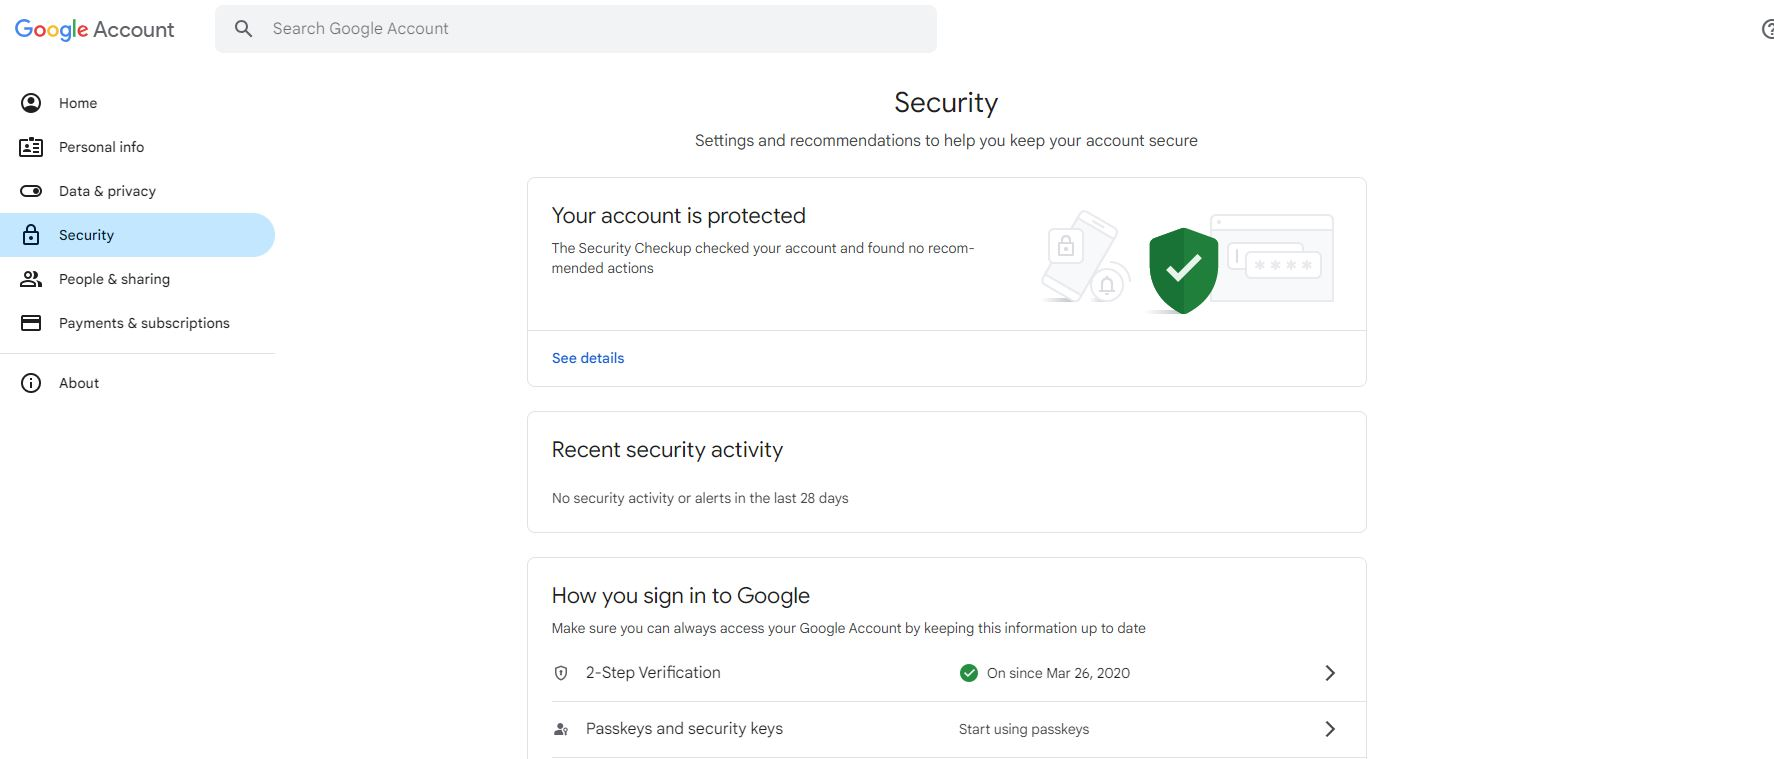
\includegraphics{images/2-step-security.JPG}

    }

    \caption{2-Step Verification}

    \end{figure}%
  \item
    Expand App passwords section (Bottom of the page) by clicking on
    that arrow

    \begin{figure}[H]

    {\centering 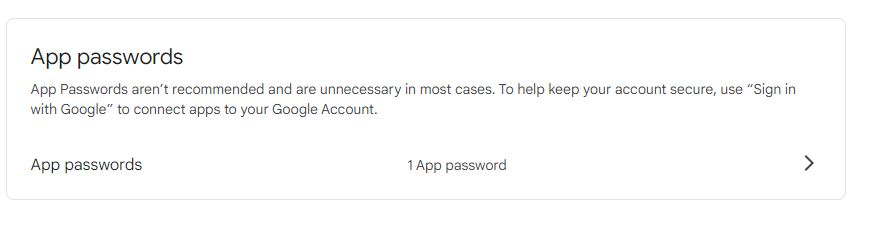
\includegraphics{images/app-pass-expand.JPG}

    }

    \caption{Click on that arrow}

    \end{figure}%
  \item
    Enter the name of the app; any name (training, python)
  \item
    Click \textbf{Create}

    \begin{figure}[H]

    {\centering 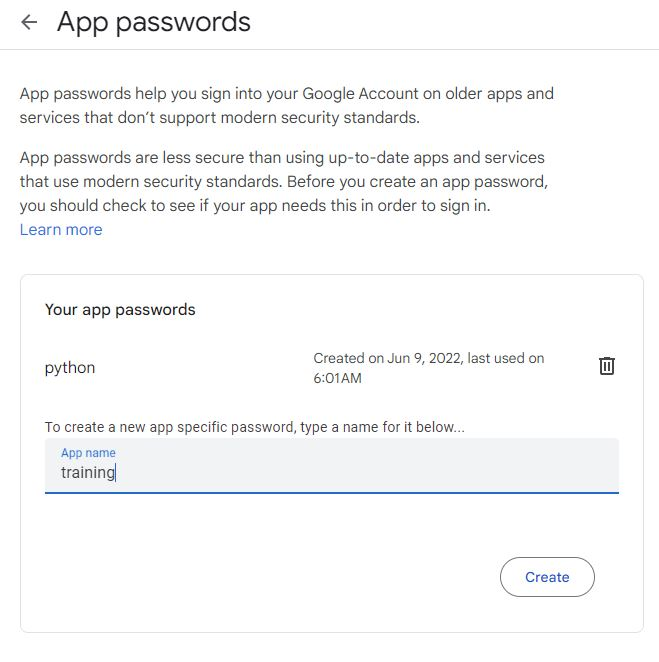
\includegraphics{images/app-pass-name.JPG}

    }

    \caption{Enter the name of the app then click Create}

    \end{figure}%
  \end{itemize}
\item
  \textbf{Use the App Password}:

  \begin{itemize}
  \item
    A 16-character app password will be displayed. Copy this password.
  \item
    Use this app password in place of your regular Gmail password in the
    application you are configuring. In our case in Python.
  \end{itemize}
\item
  \textbf{Save Your App Password}:

  \begin{itemize}
  \tightlist
  \item
    Keep this password secure, as it grants access to your Google
    account from the application. You can generate multiple app
    passwords if needed.
  \end{itemize}
\end{enumerate}

\section{Sending Updates}\label{sending-updates}

Below is a Python script for sending reports via Gmail using an app
password. This automates the process of sharing reports with
stakeholders:

\begin{Shaded}
\begin{Highlighting}[]
\ImportTok{from}\NormalTok{ email.mime.application }\ImportTok{import}\NormalTok{ MIMEApplication}
\ImportTok{from}\NormalTok{ email.mime.multipart }\ImportTok{import}\NormalTok{ MIMEMultipart}
\ImportTok{from}\NormalTok{ email.mime.text }\ImportTok{import}\NormalTok{ MIMEText}
\ImportTok{import}\NormalTok{ configparser}
\ImportTok{import}\NormalTok{ smtplib}
\ImportTok{from}\NormalTok{ os.path }\ImportTok{import}\NormalTok{ basename}
\end{Highlighting}
\end{Shaded}

\begin{Shaded}
\begin{Highlighting}[]
\NormalTok{config }\OperatorTok{=}\NormalTok{ configparser.ConfigParser()}
\NormalTok{config.read(}\StringTok{\textquotesingle{}config.ini\textquotesingle{}}\NormalTok{)}

\NormalTok{sender }\OperatorTok{=}\NormalTok{ config[}\StringTok{\textquotesingle{}email\textquotesingle{}}\NormalTok{][}\StringTok{\textquotesingle{}email\_address\textquotesingle{}}\NormalTok{]}
\NormalTok{app\_password }\OperatorTok{=}\NormalTok{ config[}\StringTok{\textquotesingle{}email\textquotesingle{}}\NormalTok{][}\StringTok{\textquotesingle{}pass\_word\textquotesingle{}}\NormalTok{]}

\NormalTok{to\_emails }\OperatorTok{=}\NormalTok{ [config[}\StringTok{\textquotesingle{}email\textquotesingle{}}\NormalTok{][}\StringTok{\textquotesingle{}recipient1\textquotesingle{}}\NormalTok{], config[}\StringTok{\textquotesingle{}email\textquotesingle{}}\NormalTok{][}\StringTok{\textquotesingle{}recipient2\textquotesingle{}}\NormalTok{],}
\NormalTok{config[}\StringTok{\textquotesingle{}email\textquotesingle{}}\NormalTok{][}\StringTok{\textquotesingle{}recipient3\textquotesingle{}}\NormalTok{]]}
\end{Highlighting}
\end{Shaded}

\begin{Shaded}
\begin{Highlighting}[]
\KeywordTok{def}\NormalTok{ send\_mail(send\_from: }\BuiltInTok{str}\NormalTok{, subject: }\BuiltInTok{str}\NormalTok{, text: }\BuiltInTok{str}\NormalTok{,}
\NormalTok{              send\_to: }\BuiltInTok{list}\NormalTok{, filess}\OperatorTok{=}\VariableTok{None}\NormalTok{):}
\NormalTok{    send\_to }\OperatorTok{=}\NormalTok{ sender }\ControlFlowTok{if} \KeywordTok{not}\NormalTok{ send\_to }\ControlFlowTok{else}\NormalTok{ send\_to}

\NormalTok{    msg }\OperatorTok{=}\NormalTok{ MIMEMultipart()}
\NormalTok{    msg[}\StringTok{\textquotesingle{}From\textquotesingle{}}\NormalTok{] }\OperatorTok{=}\NormalTok{ send\_from}
\NormalTok{    msg[}\StringTok{\textquotesingle{}To\textquotesingle{}}\NormalTok{] }\OperatorTok{=} \StringTok{\textquotesingle{}, \textquotesingle{}}\NormalTok{.join(send\_to)}
\NormalTok{    msg[}\StringTok{\textquotesingle{}Subject\textquotesingle{}}\NormalTok{] }\OperatorTok{=}\NormalTok{ subject}

\NormalTok{    msg.attach(MIMEText(text))}

    \ControlFlowTok{for}\NormalTok{ f }\KeywordTok{in}\NormalTok{ filess }\KeywordTok{or}\NormalTok{ []:}
        \ControlFlowTok{with} \BuiltInTok{open}\NormalTok{(f, }\StringTok{"rb"}\NormalTok{) }\ImportTok{as}\NormalTok{ fil:}
\NormalTok{            ext }\OperatorTok{=}\NormalTok{ f.split(}\StringTok{\textquotesingle{}.\textquotesingle{}}\NormalTok{)[}\OperatorTok{{-}}\DecValTok{1}\NormalTok{:]}
\NormalTok{            attachedfile }\OperatorTok{=}\NormalTok{ MIMEApplication(fil.read(), \_subtype}\OperatorTok{=}\NormalTok{ext)}
\NormalTok{            attachedfile.add\_header(}
                \StringTok{\textquotesingle{}content{-}disposition\textquotesingle{}}\NormalTok{, }\StringTok{\textquotesingle{}attachment\textquotesingle{}}\NormalTok{, filename}\OperatorTok{=}\NormalTok{basename(f))}
\NormalTok{        msg.attach(attachedfile)}
    \ControlFlowTok{try}\NormalTok{:}
\NormalTok{      server }\OperatorTok{=}\NormalTok{ smtplib.SMTP\_SSL(}\StringTok{\textquotesingle{}smtp.gmail.com\textquotesingle{}}\NormalTok{, }\DecValTok{465}\NormalTok{)}
\NormalTok{      server.login(sender, app\_password)}
\NormalTok{      server.sendmail(send\_from, send\_to, msg.as\_string())}
      \BuiltInTok{print}\NormalTok{(}\StringTok{"Email sent successfully!"}\NormalTok{)}
    \ControlFlowTok{except}\NormalTok{ smtplib.SMTPException }\ImportTok{as}\NormalTok{ e:}
      \BuiltInTok{print}\NormalTok{(}\SpecialStringTok{f"Failed to send email: }\SpecialCharTok{\{}\NormalTok{e}\SpecialCharTok{\}}\SpecialStringTok{"}\NormalTok{)}
    \ControlFlowTok{finally}\NormalTok{:}
\NormalTok{      server.quit()}
\end{Highlighting}
\end{Shaded}

You can write the body of the email in the script as below:

\begin{Shaded}
\begin{Highlighting}[]
\NormalTok{files\_tosend }\OperatorTok{=}\NormalTok{ [}\StringTok{"./data{-}import.qmd"}\NormalTok{]   }
    
\NormalTok{send\_mail(}
\NormalTok{  send\_from }\OperatorTok{=}\NormalTok{ sender,}
\NormalTok{  subject }\OperatorTok{=} \StringTok{"Test Email"}\NormalTok{,}
\NormalTok{  text }\OperatorTok{=} \StringTok{"Dear Moses, }\CharTok{\textbackslash{}n}\StringTok{This is a test email.}\CharTok{\textbackslash{}n\textbackslash{}r}\StringTok{ Kind regard,, }\CharTok{\textbackslash{}n}\StringTok{ Moses"}\NormalTok{,}
\NormalTok{  filess }\OperatorTok{=}\NormalTok{ files\_tosend,}
\NormalTok{  send\_to }\OperatorTok{=}\NormalTok{ to\_emails)}
\end{Highlighting}
\end{Shaded}

Another option is to store the email body in a text file, allowing you
to easily update the content without modifying the script. This approach
keeps your workflow organized and ensures that any changes to the
message can be made quickly and cleanly, maintaining a clear separation
between code and content. It's a more efficient and scalable way to
handle message updates, especially when dealing with frequent changes or
multiple stakeholders.

\begin{Shaded}
\begin{Highlighting}[]
\ControlFlowTok{with} \BuiltInTok{open}\NormalTok{(}\StringTok{\textquotesingle{}message{-}body.txt\textquotesingle{}}\NormalTok{) }\ImportTok{as}\NormalTok{ f:}
\NormalTok{  email\_body }\OperatorTok{=}\NormalTok{ f.read()}
  
  
\NormalTok{send\_mail(}
\NormalTok{  send\_from }\OperatorTok{=}\NormalTok{ sender,}
\NormalTok{  subject }\OperatorTok{=} \StringTok{"Test Email"}\NormalTok{,}
\NormalTok{  text }\OperatorTok{=}\NormalTok{ email\_body,}
\NormalTok{  filess }\OperatorTok{=}\NormalTok{ files\_tosend,}
\NormalTok{  send\_to }\OperatorTok{=}\NormalTok{ to\_emails) }
\end{Highlighting}
\end{Shaded}

\section{Track The Reports Sent}\label{track-the-reports-sent}

MySQL is the bedrock for working with relational databases. Create a
database and a table where you will be tracking your progress reports.
Working the MySQL involves the four steps below:

\begin{enumerate}
\def\labelenumi{\arabic{enumi}.}
\tightlist
\item
  Get your database connection details
\end{enumerate}

\begin{Shaded}
\begin{Highlighting}[]
\ImportTok{from}\NormalTok{ mysql.connector }\ImportTok{import}\NormalTok{ MySQLConnection}
\ImportTok{import}\NormalTok{ mysql.connector}
\ImportTok{from}\NormalTok{ mysql.connector }\ImportTok{import}\NormalTok{ Error}
\ImportTok{from}\NormalTok{ datetime }\ImportTok{import}\NormalTok{ date}


\NormalTok{config }\OperatorTok{=}\NormalTok{ configparser.ConfigParser()}
\NormalTok{config.read(}\StringTok{\textquotesingle{}config.ini\textquotesingle{}}\NormalTok{)}


\NormalTok{host\_name }\OperatorTok{=}\NormalTok{ config[}\StringTok{\textquotesingle{}mysql\textquotesingle{}}\NormalTok{][}\StringTok{\textquotesingle{}host\textquotesingle{}}\NormalTok{]}
\NormalTok{db\_user }\OperatorTok{=}\NormalTok{ config[}\StringTok{\textquotesingle{}mysql\textquotesingle{}}\NormalTok{][}\StringTok{\textquotesingle{}user\textquotesingle{}}\NormalTok{]}
\NormalTok{db }\OperatorTok{=}\NormalTok{ config[}\StringTok{\textquotesingle{}mysql\textquotesingle{}}\NormalTok{][}\StringTok{\textquotesingle{}database\textquotesingle{}}\NormalTok{]}
\NormalTok{pass\_word }\OperatorTok{=}\NormalTok{ config[}\StringTok{\textquotesingle{}mysql\textquotesingle{}}\NormalTok{][}\StringTok{\textquotesingle{}password\textquotesingle{}}\NormalTok{]}
\end{Highlighting}
\end{Shaded}

\begin{enumerate}
\def\labelenumi{\arabic{enumi}.}
\setcounter{enumi}{1}
\tightlist
\item
  Create a database
\end{enumerate}

\begin{Shaded}
\begin{Highlighting}[]
\ImportTok{from}\NormalTok{ mysql.connector }\ImportTok{import}\NormalTok{ MySQLConnection}
\ImportTok{import}\NormalTok{ mysql.connector}
\ImportTok{from}\NormalTok{ mysql.connector }\ImportTok{import}\NormalTok{ Error}

\KeywordTok{def}\NormalTok{ create\_db(dname):}
    \ControlFlowTok{try}\NormalTok{:}
        \CommentTok{\# Establish the connection}
\NormalTok{        connection }\OperatorTok{=}\NormalTok{ mysql.connector.}\ExtensionTok{connect}\NormalTok{(}
\NormalTok{            host}\OperatorTok{=}\NormalTok{host\_name,  }\CommentTok{\# e.g., \textquotesingle{}localhost\textquotesingle{} or an IP address}
\NormalTok{            user}\OperatorTok{=}\NormalTok{db\_user,}
\NormalTok{            password}\OperatorTok{=}\NormalTok{pass\_word}
\NormalTok{        )}

        \ControlFlowTok{if}\NormalTok{ connection.is\_connected():}
            \CommentTok{\# Create a cursor object}
\NormalTok{            cursor }\OperatorTok{=}\NormalTok{ connection.cursor()}

            \CommentTok{\# SQL statement to create the database}
\NormalTok{            sql\_create\_db }\OperatorTok{=} \SpecialStringTok{f"CREATE DATABASE IF NOT EXISTS }\SpecialCharTok{\{}\NormalTok{dname}\SpecialCharTok{\}}\SpecialStringTok{"}

            \CommentTok{\# Execute the query}
\NormalTok{            cursor.execute(sql\_create\_db)}
            \BuiltInTok{print}\NormalTok{(}\SpecialStringTok{f"Database \textquotesingle{}}\SpecialCharTok{\{}\NormalTok{dname}\SpecialCharTok{\}}\SpecialStringTok{\textquotesingle{} created or already exists."}\NormalTok{)}

            \CommentTok{\# Commit the transaction}
\NormalTok{            connection.commit()}
    
    \ControlFlowTok{except}\NormalTok{ Error }\ImportTok{as}\NormalTok{ e:}
        \BuiltInTok{print}\NormalTok{(}\SpecialStringTok{f"Error: }\SpecialCharTok{\{}\NormalTok{e}\SpecialCharTok{\}}\SpecialStringTok{"}\NormalTok{)}
    
    \ControlFlowTok{finally}\NormalTok{:}
        \CommentTok{\# Close the cursor and connection}
        \ControlFlowTok{if}\NormalTok{ connection.is\_connected():}
\NormalTok{            cursor.close()}
\NormalTok{            connection.close()}
            \BuiltInTok{print}\NormalTok{(}\StringTok{"MySQL connection is closed."}\NormalTok{)}
            
\NormalTok{create\_db(}\StringTok{\textquotesingle{}training\textquotesingle{}}\NormalTok{)}
\end{Highlighting}
\end{Shaded}

\begin{verbatim}
Database 'training' created or already exists.
MySQL connection is closed.
\end{verbatim}

\begin{enumerate}
\def\labelenumi{\arabic{enumi}.}
\setcounter{enumi}{2}
\tightlist
\item
  Create a table
\end{enumerate}

\begin{Shaded}
\begin{Highlighting}[]
\ImportTok{from}\NormalTok{ mysql.connector }\ImportTok{import}\NormalTok{ MySQLConnection}
\ImportTok{import}\NormalTok{ mysql.connector}
\ImportTok{from}\NormalTok{ mysql.connector }\ImportTok{import}\NormalTok{ Error}


\KeywordTok{def}\NormalTok{ create\_table(table\_name}\OperatorTok{=}\StringTok{"reports\_tracking"}\NormalTok{):}

    \ControlFlowTok{try}\NormalTok{:}
      \CommentTok{\# Establish the connection}
\NormalTok{      connection }\OperatorTok{=}\NormalTok{ mysql.connector.}\ExtensionTok{connect}\NormalTok{(}
\NormalTok{          host}\OperatorTok{=}\NormalTok{host\_name,}
\NormalTok{          user}\OperatorTok{=}\NormalTok{db\_user,}
\NormalTok{          password}\OperatorTok{=}\NormalTok{pass\_word,}
\NormalTok{          database}\OperatorTok{=}\NormalTok{db)}

      \ControlFlowTok{if}\NormalTok{ connection.is\_connected():}
          \CommentTok{\# Create a cursor object}
\NormalTok{          cursor }\OperatorTok{=}\NormalTok{ connection.cursor()}

          \CommentTok{\# SQL statement to create the table with the provided table name}
\NormalTok{          sql\_create\_table }\OperatorTok{=} \SpecialStringTok{f"""}
\SpecialStringTok{          CREATE TABLE IF NOT EXISTS }\SpecialCharTok{\{}\NormalTok{table\_name}\SpecialCharTok{\}}\SpecialStringTok{ (}
\SpecialStringTok{              id INT AUTO\_INCREMENT PRIMARY KEY,}
\SpecialStringTok{              entry\_date TIMESTAMP DEFAULT CURRENT\_TIMESTAMP,}
\SpecialStringTok{              study VARCHAR(20)}
\SpecialStringTok{          );}
\SpecialStringTok{          """}

          \CommentTok{\# Execute the query}
\NormalTok{          cursor.execute(sql\_create\_table)}
          \BuiltInTok{print}\NormalTok{(}\SpecialStringTok{f"Table \textquotesingle{}}\SpecialCharTok{\{}\NormalTok{table\_name}\SpecialCharTok{\}}\SpecialStringTok{\textquotesingle{} created or already exists."}\NormalTok{)}

          \CommentTok{\# Commit the transaction}
\NormalTok{          connection.commit()}
  
    \ControlFlowTok{except}\NormalTok{ Error }\ImportTok{as}\NormalTok{ e:}
        \BuiltInTok{print}\NormalTok{(}\SpecialStringTok{f"Error: }\SpecialCharTok{\{}\NormalTok{e}\SpecialCharTok{\}}\SpecialStringTok{"}\NormalTok{)}
    
    \ControlFlowTok{finally}\NormalTok{:}
        \CommentTok{\# Close the cursor and connection}
        \ControlFlowTok{if}\NormalTok{ connection.is\_connected():}
\NormalTok{          cursor.close()}
\NormalTok{          connection.close()}
          \BuiltInTok{print}\NormalTok{(}\StringTok{"MySQL connection is closed."}\NormalTok{)}


\NormalTok{create\_table()}
\end{Highlighting}
\end{Shaded}

\begin{verbatim}
Table 'reports_tracking' created or already exists.
MySQL connection is closed.
\end{verbatim}

\begin{enumerate}
\def\labelenumi{\arabic{enumi}.}
\setcounter{enumi}{3}
\tightlist
\item
  Insert data into the table
\end{enumerate}

\begin{Shaded}
\begin{Highlighting}[]
\ImportTok{from}\NormalTok{ mysql.connector }\ImportTok{import}\NormalTok{ MySQLConnection}
\ImportTok{import}\NormalTok{ mysql.connector}
\ImportTok{from}\NormalTok{ mysql.connector }\ImportTok{import}\NormalTok{ Error}
\ImportTok{from}\NormalTok{ datetime }\ImportTok{import}\NormalTok{ date}


\KeywordTok{def}\NormalTok{ insert\_data(study):}
\NormalTok{    c\_date }\OperatorTok{=}\NormalTok{ date.today()}
    \ControlFlowTok{try}\NormalTok{:}
        
        \CommentTok{\# Establish the connection}
\NormalTok{        connection }\OperatorTok{=}\NormalTok{ mysql.connector.}\ExtensionTok{connect}\NormalTok{(}
\NormalTok{            host}\OperatorTok{=}\NormalTok{host\_name,  }\CommentTok{\# e.g., \textquotesingle{}localhost\textquotesingle{} or an IP address}
\NormalTok{            user}\OperatorTok{=}\NormalTok{db\_user,}
\NormalTok{            password}\OperatorTok{=}\NormalTok{pass\_word,}
\NormalTok{            database}\OperatorTok{=}\NormalTok{db)     }

        \ControlFlowTok{if}\NormalTok{ connection.is\_connected():}
                \BuiltInTok{print}\NormalTok{(}\StringTok{"Connected to MySQL database"}\NormalTok{)}

                \CommentTok{\# Create a cursor object}
\NormalTok{                cursor }\OperatorTok{=}\NormalTok{ connection.cursor()}

                \CommentTok{\# SQL INSERT statement}
\NormalTok{                sql\_insert\_query }\OperatorTok{=} \StringTok{"""INSERT INTO reports\_tracking (entry\_date, study)}
\StringTok{                                    VALUES (}\SpecialCharTok{\%s}\StringTok{, }\SpecialCharTok{\%s}\StringTok{)"""}
                \CommentTok{\# Values to insert}
\NormalTok{                values\_to\_insert }\OperatorTok{=}\NormalTok{ (c\_date, study)}

                \CommentTok{\# Execute the query}
\NormalTok{                cursor.execute(sql\_insert\_query, values\_to\_insert)}

                \CommentTok{\# Commit the transaction}
\NormalTok{                connection.commit()}
                \BuiltInTok{print}\NormalTok{(}\StringTok{"Data inserted successfully"}\NormalTok{)}

    \ControlFlowTok{except}\NormalTok{ Error }\ImportTok{as}\NormalTok{ e:}
        \BuiltInTok{print}\NormalTok{(}\SpecialStringTok{f"Error: }\SpecialCharTok{\{}\NormalTok{e}\SpecialCharTok{\}}\SpecialStringTok{"}\NormalTok{)}
    \ControlFlowTok{finally}\NormalTok{:}

        \CommentTok{\# Close the cursor and connection}
        \ControlFlowTok{if}\NormalTok{ connection.is\_connected():}
\NormalTok{            cursor.close()}
\NormalTok{            connection.close()}

\CommentTok{\# Call the function to insert data}
\NormalTok{insert\_data(}\StringTok{"Training"}\NormalTok{)}
\end{Highlighting}
\end{Shaded}

\begin{verbatim}
Connected to MySQL database
Data inserted successfully
\end{verbatim}

To avoid sending reports multiple times in a day, you can leverage the
MySQL databases. First, fetch the data from the MySQL server and check
if the report has been updated. If it hasn't been sent that day, proceed
to send it. We will update our \texttt{send\_mail} function to ensure we
track our progress reports.

\begin{Shaded}
\begin{Highlighting}[]
\ImportTok{from}\NormalTok{ mysql.connector }\ImportTok{import}\NormalTok{ MySQLConnection}
\ImportTok{import}\NormalTok{ mysql.connector}
\ImportTok{from}\NormalTok{ mysql.connector }\ImportTok{import}\NormalTok{ Error}
\ImportTok{from}\NormalTok{ datetime }\ImportTok{import}\NormalTok{ date}

\KeywordTok{def}\NormalTok{ fetch\_data():}
  \ControlFlowTok{try}\NormalTok{:}
        \CommentTok{\# Establish the connection}
\NormalTok{        connection }\OperatorTok{=}\NormalTok{ mysql.connector.}\ExtensionTok{connect}\NormalTok{(}
\NormalTok{            host}\OperatorTok{=}\NormalTok{host\_name,  }\CommentTok{\# e.g., \textquotesingle{}localhost\textquotesingle{} or an IP address}
\NormalTok{            user}\OperatorTok{=}\NormalTok{db\_user,}
\NormalTok{            password}\OperatorTok{=}\NormalTok{pass\_word,}
\NormalTok{            database}\OperatorTok{=}\NormalTok{db)     }

        \ControlFlowTok{if}\NormalTok{ connection.is\_connected():}
          
                \CommentTok{\# Create a cursor object}
\NormalTok{                cursor }\OperatorTok{=}\NormalTok{ connection.cursor()}

                \CommentTok{\# {-}{-}{-}{-} Pull the entry\_date from the database}

\NormalTok{                cursor.execute(}\StringTok{"SELECT entry\_date FROM reports\_tracking"}\NormalTok{)}
                
\NormalTok{                reportcentries }\OperatorTok{=}\NormalTok{ cursor.fetchall()}
                
\NormalTok{                entries }\OperatorTok{=}\NormalTok{ [j.date() }\ControlFlowTok{for}\NormalTok{ i }\KeywordTok{in}\NormalTok{ reportcentries }\ControlFlowTok{for}\NormalTok{ j }\KeywordTok{in}\NormalTok{ i]}
                
                \ControlFlowTok{return}\NormalTok{ entries}

                \CommentTok{\# Commit the transaction}
\NormalTok{                connection.commit()}
                \BuiltInTok{print}\NormalTok{(}\StringTok{"Data inserted successfully"}\NormalTok{)}

  \ControlFlowTok{except}\NormalTok{ Error }\ImportTok{as}\NormalTok{ e:}
        \BuiltInTok{print}\NormalTok{(}\SpecialStringTok{f"Error: }\SpecialCharTok{\{}\NormalTok{e}\SpecialCharTok{\}}\SpecialStringTok{"}\NormalTok{)}
  \ControlFlowTok{finally}\NormalTok{:}
        
        \CommentTok{\# Close the cursor and connection}
        \ControlFlowTok{if}\NormalTok{ connection.is\_connected():}
\NormalTok{            cursor.close()}
\NormalTok{            connection.close()}
\end{Highlighting}
\end{Shaded}

Update the \texttt{send\_mail} function

\begin{Shaded}
\begin{Highlighting}[]
\KeywordTok{def}\NormalTok{ send\_mail(send\_from: }\BuiltInTok{str}\NormalTok{, subject: }\BuiltInTok{str}\NormalTok{, text: }\BuiltInTok{str}\NormalTok{,}
\NormalTok{              send\_to: }\BuiltInTok{list}\NormalTok{, filess}\OperatorTok{=}\VariableTok{None}\NormalTok{):}
\NormalTok{    send\_to }\OperatorTok{=}\NormalTok{ sender }\ControlFlowTok{if} \KeywordTok{not}\NormalTok{ send\_to }\ControlFlowTok{else}\NormalTok{ send\_to}

\NormalTok{    msg }\OperatorTok{=}\NormalTok{ MIMEMultipart()}
\NormalTok{    msg[}\StringTok{\textquotesingle{}From\textquotesingle{}}\NormalTok{] }\OperatorTok{=}\NormalTok{ send\_from}
\NormalTok{    msg[}\StringTok{\textquotesingle{}To\textquotesingle{}}\NormalTok{] }\OperatorTok{=} \StringTok{\textquotesingle{}, \textquotesingle{}}\NormalTok{.join(send\_to)}
\NormalTok{    msg[}\StringTok{\textquotesingle{}Subject\textquotesingle{}}\NormalTok{] }\OperatorTok{=}\NormalTok{ subject}

\NormalTok{    msg.attach(MIMEText(text))}

    \ControlFlowTok{for}\NormalTok{ f }\KeywordTok{in}\NormalTok{ filess }\KeywordTok{or}\NormalTok{ []:}
        \ControlFlowTok{with} \BuiltInTok{open}\NormalTok{(f, }\StringTok{"rb"}\NormalTok{) }\ImportTok{as}\NormalTok{ fil:}
\NormalTok{            ext }\OperatorTok{=}\NormalTok{ f.split(}\StringTok{\textquotesingle{}.\textquotesingle{}}\NormalTok{)[}\OperatorTok{{-}}\DecValTok{1}\NormalTok{:]}
\NormalTok{            attachedfile }\OperatorTok{=}\NormalTok{ MIMEApplication(fil.read(), \_subtype}\OperatorTok{=}\NormalTok{ext)}
\NormalTok{            attachedfile.add\_header(}
                \StringTok{\textquotesingle{}content{-}disposition\textquotesingle{}}\NormalTok{, }\StringTok{\textquotesingle{}attachment\textquotesingle{}}\NormalTok{, filename}\OperatorTok{=}\NormalTok{basename(f))}
\NormalTok{        msg.attach(attachedfile)}
    \ControlFlowTok{try}\NormalTok{:}
\NormalTok{      server }\OperatorTok{=}\NormalTok{ smtplib.SMTP\_SSL(}\StringTok{\textquotesingle{}smtp.gmail.com\textquotesingle{}}\NormalTok{, }\DecValTok{465}\NormalTok{)}
\NormalTok{      server.login(sender, app\_password)}
\NormalTok{      server.sendmail(send\_from, send\_to, msg.as\_string())}
\NormalTok{      insert\_data(}\StringTok{"Training"}\NormalTok{)}
      \BuiltInTok{print}\NormalTok{(}\StringTok{"Email sent successfully!"}\NormalTok{)}
    \ControlFlowTok{except}\NormalTok{ smtplib.SMTPException }\ImportTok{as}\NormalTok{ e:}
      \BuiltInTok{print}\NormalTok{(}\SpecialStringTok{f"Failed to send email: }\SpecialCharTok{\{}\NormalTok{e}\SpecialCharTok{\}}\SpecialStringTok{"}\NormalTok{)}
    \ControlFlowTok{finally}\NormalTok{:}
\NormalTok{      server.quit()}
\end{Highlighting}
\end{Shaded}

Send updates if not sent

\begin{Shaded}
\begin{Highlighting}[]
\ControlFlowTok{with} \BuiltInTok{open}\NormalTok{(}\StringTok{\textquotesingle{}message{-}body.txt\textquotesingle{}}\NormalTok{) }\ImportTok{as}\NormalTok{ f:}
\NormalTok{  email\_body }\OperatorTok{=}\NormalTok{ f.read()}
  
\NormalTok{entries }\OperatorTok{=}\NormalTok{ fetch\_data()}
\NormalTok{date\_today }\OperatorTok{=}\NormalTok{ date.today()}

\ControlFlowTok{if}\NormalTok{ date\_today }\KeywordTok{not} \KeywordTok{in}\NormalTok{ entries:}
\NormalTok{  send\_mail(}
\NormalTok{    send\_from }\OperatorTok{=}\NormalTok{ sender,}
\NormalTok{    subject }\OperatorTok{=} \StringTok{"Test Email"}\NormalTok{,}
\NormalTok{    text }\OperatorTok{=}\NormalTok{ email\_body,}
\NormalTok{    filess }\OperatorTok{=}\NormalTok{ files\_tosend,}
\NormalTok{    send\_to }\OperatorTok{=}\NormalTok{ to\_emails) }
\ControlFlowTok{else}\NormalTok{:}
  \BuiltInTok{print}\NormalTok{(}\StringTok{"You have sent the updates today"}\NormalTok{)}
\end{Highlighting}
\end{Shaded}

\begin{verbatim}
You have sent the updates today
\end{verbatim}

\section{Summary}\label{summary-3}

Once reports are generated, the next step is ensuring timely
distribution to stakeholders. Automating this process with Python and
Gmail enhances efficiency by reducing manual effort. By using a Gmail
app password, which offers a secure way to integrate Gmail into
applications without compromising your main account password, you ensure
smooth, secure, and reliable email distribution.

The script provided sends reports as email attachments. It reads the
sender's credentials and recipients' information from a configuration
file (\texttt{config.ini}). The function \texttt{send\_mail} handles the
email composition and attachments, sending them securely via Gmail's
SMTP server. In the event of failure, the script uses a
\texttt{try-except} block to catch errors and ensures the server
connection is closed.

An additional recommendation is to store the email body in a separate
text file for easier management, especially when frequently updating the
content for various stakeholders. This keeps the script clean and
maintainable.

We finalized the script to ensure updates are sent only if they haven't
been previously sent.

\bookmarksetup{startatroot}

\chapter{Batch Scripting}\label{batch-scripting}

\section{Introduction}\label{introduction-7}

A~Batch Script~is text file containing lines with commands that get
executed in sequence by the Microsoft command interpreter (cmd.exe).
Batch scripts~files have the special extension BAT (\texttt{.bat}) or
CMD (\texttt{.cmd}). This type of file is recognized by the Operating
System and executed through an interface (called shell) provided by a
system file called the~command interpreter. Batch scripting is a
powerful way to automate data management workflows by allowing you to
write simple scripts that can execute multiple commands. It is
especially useful for handling repetitive tasks such as file
organization, renaming, backups, and even scheduling automated data
processing. With batch scripting, you can improve efficiency, reduce
manual work, and ensure consistency in your data management processes. I
created a batch script to automate the entire data management workflow.

\section{Why Batch Scripts}\label{why-batch-scripts}

There are tons of reasons why I prefer batch script. A few of them are
list below:

\begin{itemize}
\item
  \textbf{Automation:} Batch scripts automate repetitive tasks, saving
  time and reducing manual effort.
\item
  \textbf{Efficiency:} They streamline processes, allowing multiple
  commands to run sequentially with minimal intervention.
\item
  \textbf{Consistency:} Ensure uniform execution of tasks, reducing the
  chances of errors.
\item
  \textbf{Flexibility:} Batch scripts can be customized to handle
  various tasks such as backups, file management, and data processing.
\item
  \textbf{Integration:} Easily integrate with other tools or scripts to
  enhance data workflows.
\item
  \textbf{Cost-Effective:} No need for additional software; batch
  scripting works on most operating systems.
\item
  \textbf{Simplicity:} Batch scripts are easy to write and execute,
  requiring minimal setup.
\end{itemize}

\section{Batch Script for Automation}\label{batch-script-for-automation}

Below is a simple example of how you can write your batch script:

\begin{Shaded}
\begin{Highlighting}[]
\ControlFlowTok{with} \BuiltInTok{open}\NormalTok{(}\StringTok{\textquotesingle{}scripts/training{-}batch.bat\textquotesingle{}}\NormalTok{) }\ImportTok{as}\NormalTok{ f:}
\NormalTok{  batch }\OperatorTok{=}\NormalTok{ f.read()}
  
\BuiltInTok{print}\NormalTok{(batch)}
\end{Highlighting}
\end{Shaded}

\begin{verbatim}
:: ----------------------------- Begin Header -----------------------------------
:: Name of the batch file : training-batch.bat
::
:: Purpose : Automate the pulling of data from the server and run the R scripts that clean data
::
:: Input  :  
::
:: Output : Updated datasets
::          Updated reports
::
::
:: Authors : Moses Otieno
::
::
:: Contact Email : mosotieno25@gmail.com
::
::
:: First version : 15 October 2024
::
::
:: Reviewed :
::
:: ----------------------------- End Header--------------------------------------


echo "Downloading and preparing project data..."

:: Change the directory appropriately

D:
cd "D:\InterestingTasks\data-mngmt\scripts"


:: Run the python script to pull the data from the server

python "download_data.py"

:: Wait the download

timeout /t 3  /nobreak  

Rscript "master.R"



\end{verbatim}

\section{Automating Batch Script}\label{automating-batch-script}

Throughout this journey, we've emphasized the importance of automation
in streamlining our workflows. Now that we've developed a robust batch
script, the next step is to automate its execution.

\begin{itemize}
\item
  \textbf{For Windows Users}: Utilize the Task Scheduler to run your
  batch script at specified intervals or triggers. This tool allows you
  to schedule tasks to run automatically, ensuring your processes are
  carried out without manual intervention.
\item
  \textbf{For Linux Users}: Leverage \texttt{cron}, a time-based job
  scheduler, to automate your batch script execution. You can set up
  cron jobs to run your scripts at designated times or intervals,
  enhancing efficiency and reliability.
\item
  \textbf{For Mac Users}: Use \texttt{launchd}, the built-in service
  management framework, to automate your batch script. You can create a
  \texttt{.plist} file to define when and how your script should run,
  allowing for seamless execution of tasks at specified times or events.
\end{itemize}

By implementing these scheduling tools, you can maintain a seamless
workflow, allowing you to focus on other important tasks while your
scripts run automatically. I will do a qucik run on how to schedule
tasks on Windows.

\subsection{Scheduling Tasks on
Windows}\label{scheduling-tasks-on-windows}

\begin{itemize}
\item
  \textbf{Open Task Scheduler}:

  \begin{itemize}
  \item
    Press \texttt{Windows\ +\ R} to open the Run dialog.
  \item
    Type \texttt{taskschd.msc} and hit \texttt{Enter}.
  \item
    You may be requested to key in your user password. Do so.
  \end{itemize}
\item
  \textbf{Create a New Task}:

  \begin{itemize}
  \item
    In the Task Scheduler window, click on \textbf{``Create Basic
    Task''} in the right-hand pane.

    \begin{figure}[H]

    {\centering 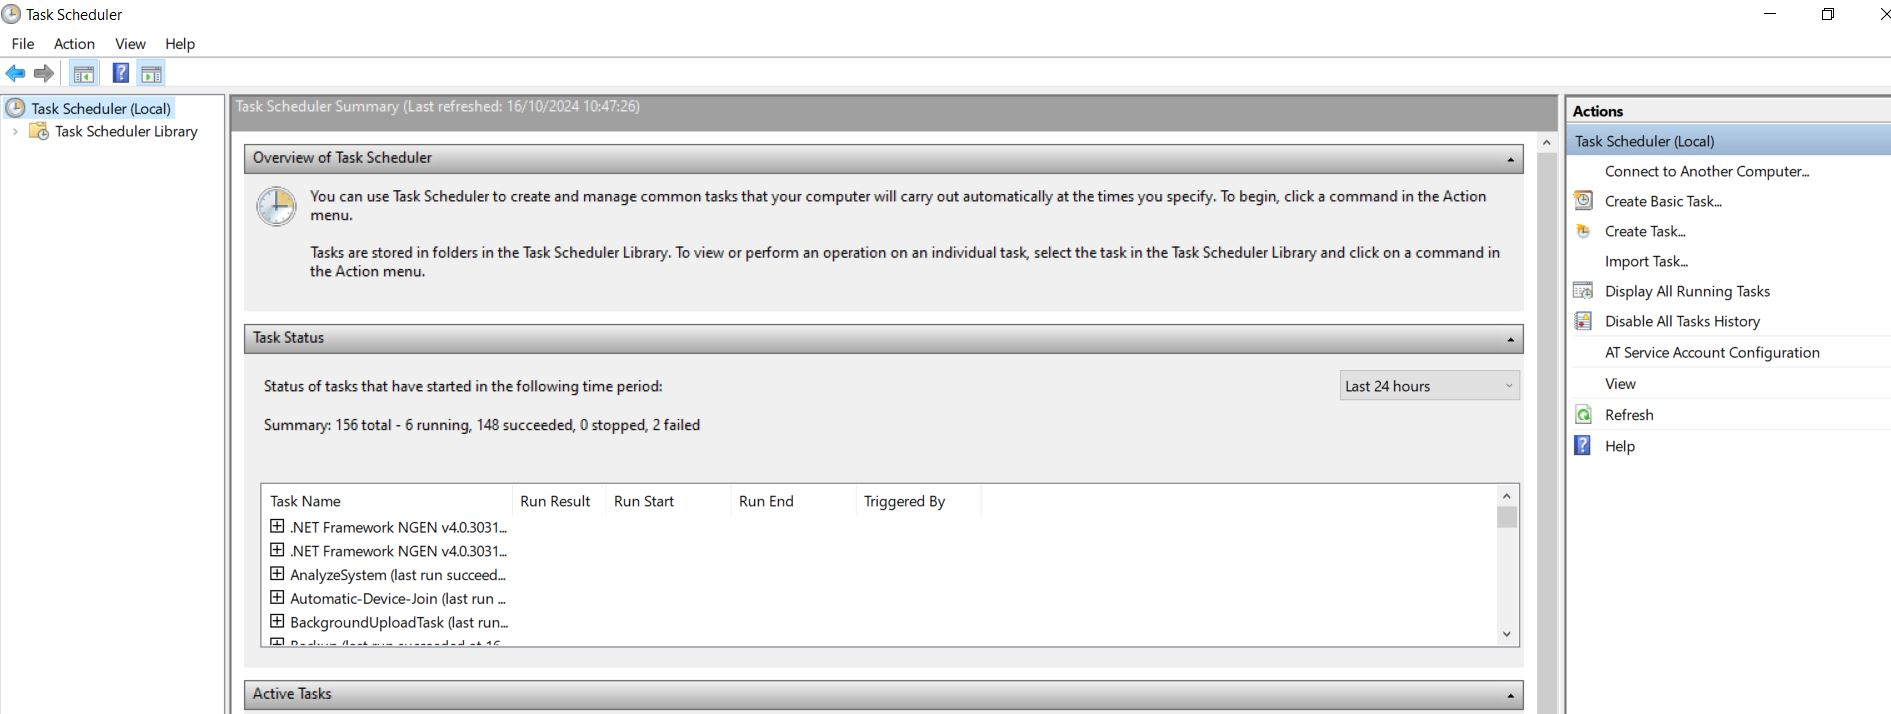
\includegraphics[width=6.54167in,height=\textheight]{images/task-schedule-basic-01.JPG}

    }

    \caption{Click Create Basic Task}

    \end{figure}%
  \end{itemize}
\item
  \textbf{Name Your Task}:

  \begin{itemize}
  \item
    Enter a name and description for your task, then click
    \textbf{``Next.''}

    \begin{figure}[H]

    {\centering 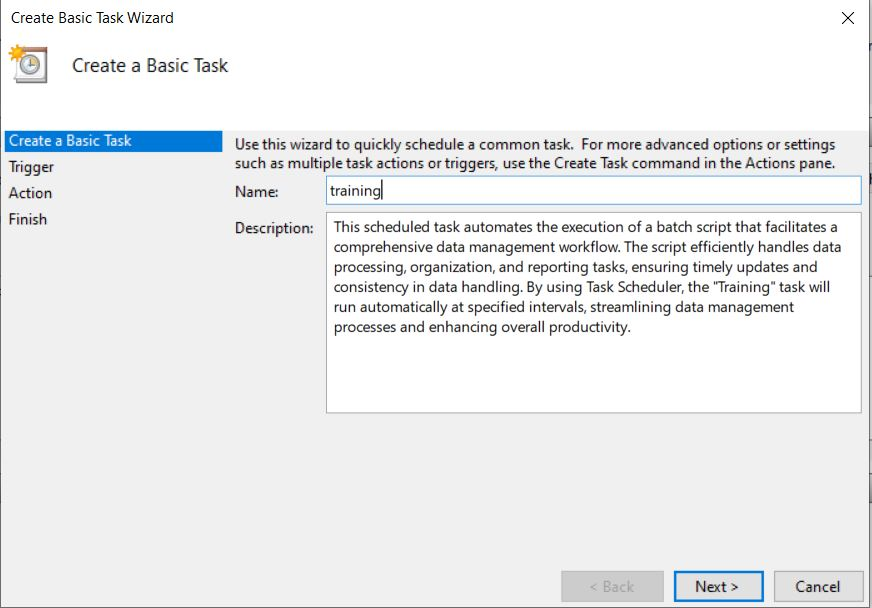
\includegraphics{images/name_desc_task.JPG}

    }

    \caption{Name and description of task}

    \end{figure}%
  \end{itemize}
\item
  \textbf{Choose a Trigger}:

  \begin{itemize}
  \item
    Select when you want the task to start (e.g., Daily, Weekly, One
    time, etc.) and click \textbf{``Next.''}
  \item
    Configure the trigger details (e.g., time, frequency) and click
    \textbf{``Next.''}
  \end{itemize}
\item
  \textbf{Choose an Action}:

  \begin{itemize}
  \tightlist
  \item
    Select \textbf{``Start a program''} and click \textbf{``Next.''}
  \end{itemize}
\item
  \textbf{Select Your Batch Script}:

  \begin{itemize}
  \item
    Click \textbf{``Browse''} to locate your batch script file.
  \item
    Optionally, you can add arguments or specify the ``Start in''
    directory.
  \item
    Click \textbf{``Next.''}
  \end{itemize}
\item
  \textbf{Review and Finish}:

  \begin{itemize}
  \item
    Review your task settings. If everything looks good, click
    \textbf{``Finish.''}

    \begin{figure}[H]

    {\centering 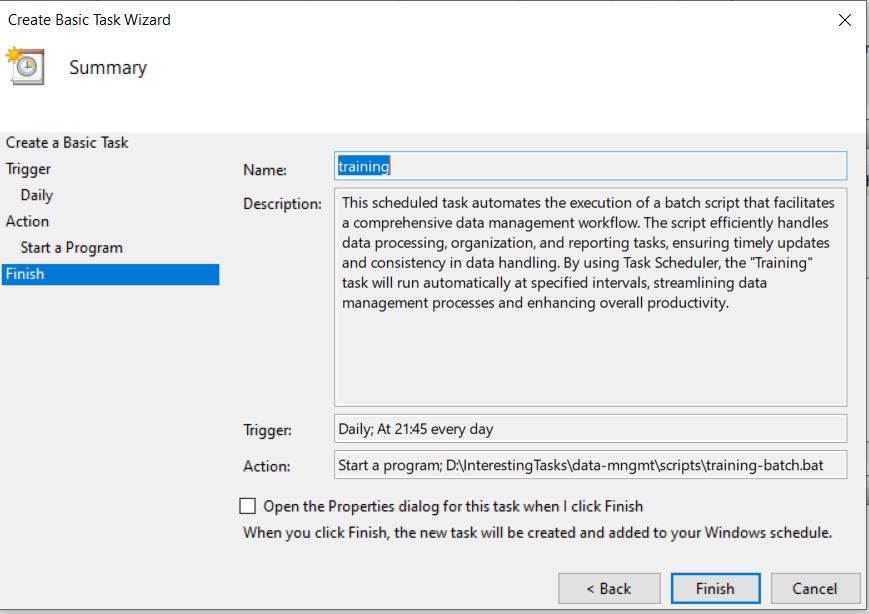
\includegraphics{images/taskscheduler-summary.JPG}

    }

    \caption{Summary of task scheduled}

    \end{figure}%
  \end{itemize}
\item
  \textbf{Manage Your Task}:

  \begin{itemize}
  \tightlist
  \item
    To edit or manage your scheduled task, locate it in the Task
    Scheduler Library. Right-click on the task for options like
    \textbf{Run, End, or Delete}.
  \end{itemize}
\end{itemize}

\begin{figure}[H]

{\centering 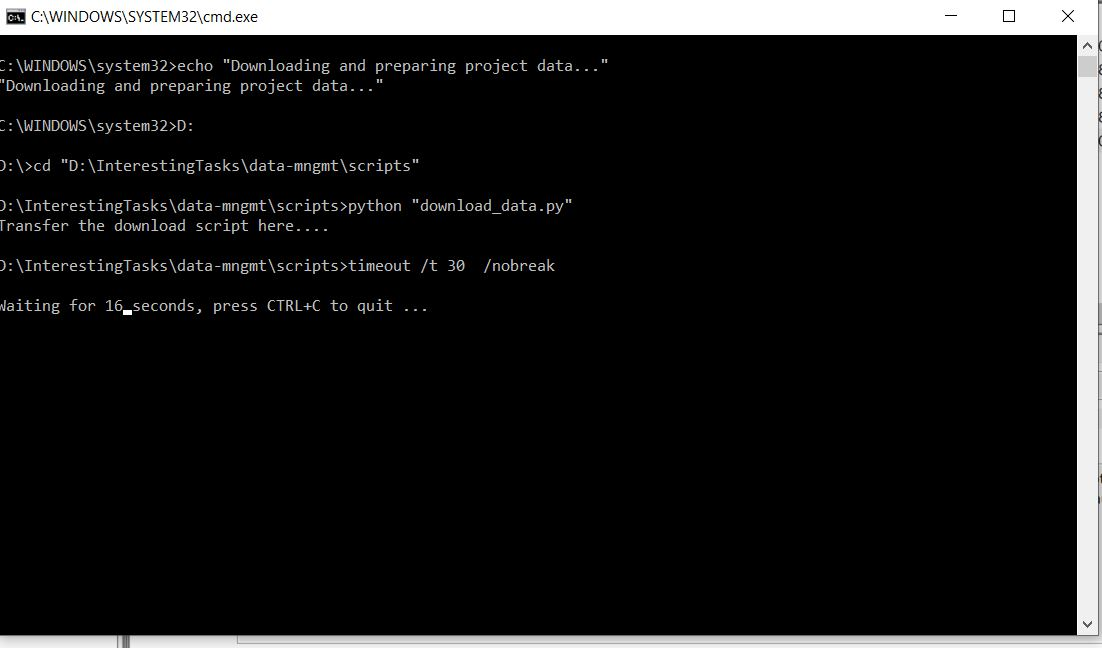
\includegraphics{images/task_running.JPG}

}

\caption{The task is running!}

\end{figure}%

Voila! We have done it!!!!

\section{Summary}\label{summary-4}

In this section, we explored the significance of batch scripting in
creating an efficient data management workflow. Batch scripts automate
repetitive tasks, allowing users to execute multiple commands without
manual intervention, thus enhancing productivity and minimizing errors.
We discussed various reasons for preferring batch scripts, including
their simplicity, efficiency, and ability to manage complex workflows
seamlessly.

We also highlighted the importance of task schedulers for automating
batch scripts, with specific instructions for Windows users to schedule
tasks effectively. For Linux users, we mentioned using cron jobs, and
for Mac users, we suggested utilizing Automator or the launchd system
for similar task automation.

By integrating batch scripts and task schedulers into our data
management workflow, we streamline processes, improve consistency, and
ultimately crown the workflow with a robust and automated solution. For
more details about batch scripting check
\href{https://tutorialreference.com/batch-scripting/batch-script-tutorial}{here}.

\bookmarksetup{startatroot}

\chapter*{References}\label{references}
\addcontentsline{toc}{chapter}{References}

\markboth{References}{References}

\phantomsection\label{refs}
\begin{CSLReferences}{0}{1}
\bibitem[\citeproctext]{ref-briney}
\CSLLeftMargin{1. }%
\CSLRightInline{Briney K. \emph{Data Management for Researchers:
Organize, Maintain and Share Your Data for Research Success}. Pelagic
Publishing}

\bibitem[\citeproctext]{ref-sweigartal2019}
\CSLLeftMargin{2. }%
\CSLRightInline{Sweigart, Al. \emph{Automate the Boring Stuff with
Python: Practical Programming for Total Beginners}. 2nd ed. No Starch
Press; 2019.}

\bibitem[\citeproctext]{ref-mckinneywes2018}
\CSLLeftMargin{3. }%
\CSLRightInline{McKinney, Wes. \emph{Python for Data Analysis: Data
Wrangling with Pandas, NumPy, and IPython}. 2nd ed. O'Reilly Media, Inc;
2018. \url{https://wesmckinney.com/book/}}

\bibitem[\citeproctext]{ref-wickhamhadley2023}
\CSLLeftMargin{4. }%
\CSLRightInline{Wickham, Hadley, Mine Çetinkaya-Rundel, Garrett
Grolemund. \emph{R for Data Science: Import, Tidy, Transform, Visualize,
and Model Data}. 2nd ed.; 2023.}

\end{CSLReferences}




\end{document}
